% !TEX root = ../Elements.tex
% Greek and English text last checked 14/03/2013
%%%%%%
% BOOK 2
%%%%%%
\pdfbookmark[0]{Book 2}{book2}
\pagestyle{empty}
\begin{center}
{\Huge ELEMENTS BOOK 2}\\
\spa\spa\spa
{\huge\it Fundamentals of Geometric Algebra}
\end{center}
%\vspace{2cm}
%\epsfysize=5in
%\centerline{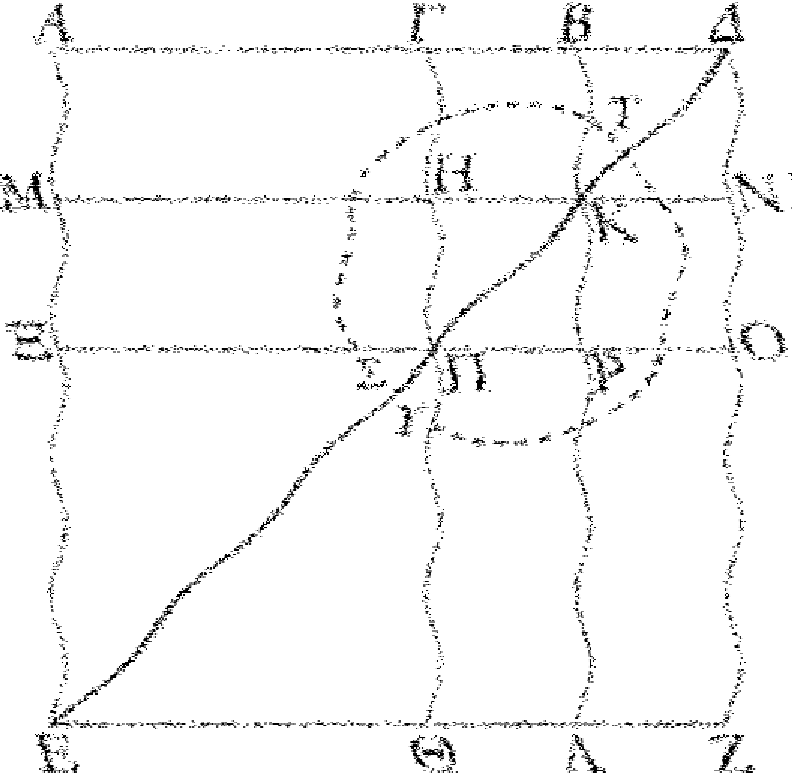
\includegraphics{Book02/front.eps}}
\newpage

%%%%%%%
% Definitions
%%%%%%%
\pdfbookmark[1]{Definitions}{def2}
\pagestyle{fancy}
\cfoot{\gr{\kern -.7pt }}
\lhead{\large\gr{ΣΤΟΙΘΕΙΩΝ \kern -.7pt {2}.}}
\rhead{\large ELEMENTS BOOK 2}
\begin{Parallel}{}{} 
\ParallelLText{
\begin{center}
\large{\gr{<'Οροι}.}
\end{center}
\vspace*{-7pt}

\ggn{1}.~\gr{Πᾶν παραλληλόγραμμον ὀρθογώνιον περιέθεσθαι λέγεται ὑπὸ δύο τῶν τὴν ὀρθὴν γωνίαν περιεθουσῶν εὐθειῶν.}

\ggn{2}.~\gr{Παντὸξ δὲ παραλληλογράμμου θωρίου τῶν περὶ τὴν διάμετρον
α\kern -.7pt  ὐτοῦ παραλληλογράμμων <ὲν ὁποιονοῦν σὺν τοῖξ δυσὶ παραπληρώμασι γνώμων καλείσθω.}}

\ParallelRText{
\begin{center}
{\large Definitions}
\end{center}

1.~Any rectangular parallelogram is said to be contained by the two
 straight-lines containing the right-angle.
 
2.~And in any parallelogrammic figure, let any one whatsoever of the parallelograms about
its diagonal,  (taken) with its two complements, be called
a gnomon.}
\end{Parallel}

%%%%%%
% Prop 2.1
%%%%%%
\pdfbookmark[1]{Proposition 2.1}{pdf2.1}
\begin{Parallel}{}{} 
\ParallelLText{
\begin{center}
{\large \ggn{1}.}
\end{center}\vspace*{-7pt}

\gr{Ἐὰν >ῶσι δύο εὐθεῖαι, τμ\kern -.7pt  ηθῆ| δὲ ἡ ἑτέρα α\kern -.7pt  ὐτῶν εἰξ ὁσαδηποτοῦν τμ\kern -.5pt  ήματα, τὸ περιεχόμενον ὀρθογώνιον ὑπὸ τῶν δύο εὐθειῶν >ίσον ἐστὶ τοῖξ ὑπό τε τῆξ ἀτμ\kern -.3pt  ήτου καὶ ἑκάστου τῶν τμ\kern -.7pt  ημάτων περιεθομένοιξ ὀρθογωνίοιξ.}\\

\epsfysize=2.2in
\centerline{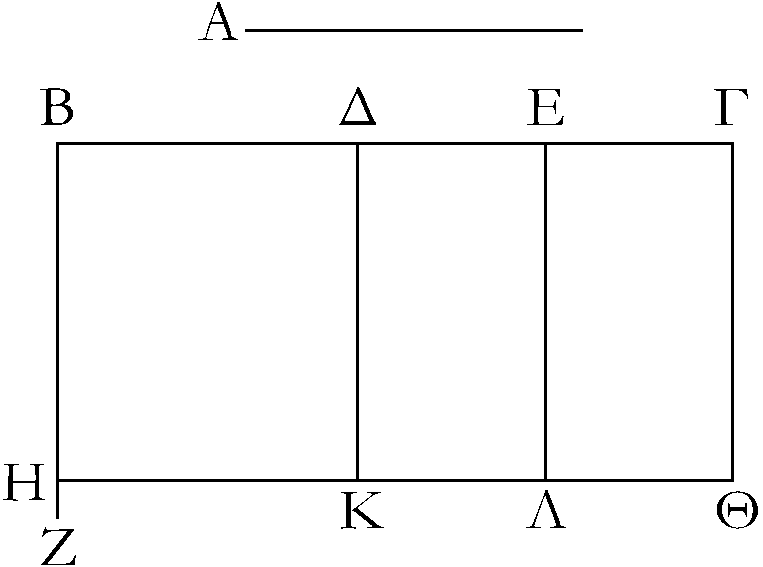
\includegraphics{Book02/fig01g.eps}}

\gr{>'Εστωσαν δύο εὐθεῖαι αἱ Α, ΒΓ, καὶ τετμ\kern -.7pt  ήσθω ἡ ΒΓ, ὡξ >έτυθεν, κατὰ τὰ Δ, Ε σημεῖα; λέγω, <ότι τὸ ὑπὸ τῶν Α, ΒΓ περιεθομένον ὀρθογώνιον >ίσον ἐστὶ τῶ| τε ὑπὸ τῶν Α, ΒΔ περιεθομένῳ ὀρθογωνίῳ καὶ τῶ| ὑπὸ τῶν Α, ΔΕ καὶ >έτι τῶ| ὑπὸ τῶν Α,
ΕΓ.}

\gr{>'Ηθθω γὰρ ἀπὸ τοῦ Β τῆ| ΒΓ πρὸξ ὀρθὰξ ἡ ΒΖ, καὶ κείσθω
τῆ| Α >ίση ἡ ΒΗ, καὶ διὰ μὲν τοῦ Η τῆ| ΒΓ παράλληλοξ >ήθθω ἡ ΗJ, διὰ δὲ τῶν Δ, Ε, Γ τῆ| ΒΗ παράλληλοι >ήθθωσαν αἱ ΔΚ, ΕΛ, ΓJ.}

\gr{>'Ισον δή ἐστι τὸ ΒJ τοῖξ ΒΚ, ΔΛ, ΕJ. καί ἐστι τὸ μὲν ΒJ τὸ ὑπὸ τῶν Α, ΒΓ; περιέθεται μὲν γὰρ ὑπὸ τῶν ΗΒ, ΒΓ, >ίση δὲ ἡ ΒΗ τῆ| Α; τὸ δὲ ΒΚ τὸ ὑπὸ τῶν Α, ΒΔ; περιέθεται μὲν γὰρ ὑπὸ τῶν ΗΒ, ΒΔ, >ίση δὲ ἡ ΒΗ τῆ| Α. τὸ δὲ ΔΛ τὸ ὑπὸ τῶν Α, ΔΕ; >ίση γὰρ ἡ ΔΚ, τουτέστιν ἡ ΒΗ, τῆ| Α. καὶ >έτι ὁμοίωξ τὸ ΕJ τὸ ὑπὸ τῶν Α, ΕΓ; τὸ >άρα ὑπὸ τῶν Α, ΒΓ >ίσον ἐστὶ τῶ| τε ὑπὸ Α, ΒΔ καὶ
τῶ| ὑπὸ Α, ΔΕ καὶ >έτι τῶ| ὑπὸ Α, ΕΓ.}

\gr{Ἐὰν >άρα  >ῶσι δύο εὐθεῖαι, τμ\kern -.7pt  ηθῆ| δὲ ἡ ἑτέρα α\kern -.7pt  ὐτῶν εἰξ ὁσαδηποτοῦν τμ\kern -.5pt  ήματα, τὸ περιεχόμενον ὀρθογώνιον ὑπὸ τῶν δύο εὐθειῶν >ίσον ἐστὶ τοῖξ ὑπό τε τῆξ ἀτμ\kern -.3pt  ήτου καὶ ἑκάστου τῶν τμ\kern -.7pt  ημάτων περιεθομένοιξ ὀρθογωνίοιξ; <όπερ >έδει δεῖχαι.}}

\ParallelRText{
\begin{center}
{\large Proposition 1$^\dag$}
\end{center}

If there are two straight-lines, and one of them is cut into any number of pieces whatsoever, (then) the rectangle contained by the two straight-lines is
equal to the (sum of the) rectangles contained by the uncut (straight-line), and every one of the pieces (of the cut straight-line).

\epsfysize=2.2in
\centerline{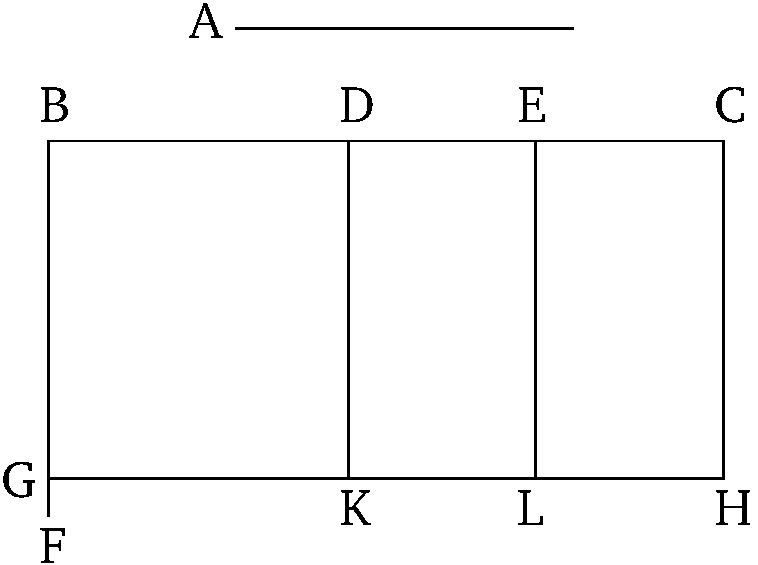
\includegraphics{Book02/fig01e.eps}}

Let $A$ and $BC$ be the two straight-lines, and let $BC$ be cut, at random,
at points $D$ and $E$. I say that the rectangle contained by $A$ and $BC$ is equal
to the rectangle(s) contained by $A$ and $BD$, by $A$ and $DE$, and, finally, by $A$ and
$EC$.

For let $BF$ be drawn from point $B$, at right-angles to $BC$ [Prop.~1.11],
and let $BG$ be made equal to $A$ [Prop.~1.3], and let $GH$ be drawn through
(point) $G$, parallel to $BC$ [Prop.~1.31], and let $DK$, $EL$, and $CH$ be drawn through (points) $D$, $E$, and $C$ (respectively), parallel to $BG$ [Prop.~1.31].

So the (rectangle) $BH$ is equal to the (rectangles) $BK$, $DL$, and $EH$. And
$BH$ is  the (rectangle contained) by $A$ and $BC$. For it is contained by $GB$ and $BC$, and $BG$ (is) equal to $A$. And  $BK$ (is) the (rectangle contained) by $A$ and $BD$.
For it is contained by $GB$ and $BD$, and $BG$ (is) equal to $A$. And $DL$ (is) the (rectangle contained) by $A$ and $DE$.
For $DK$, that is to say $BG$ [Prop.~1.34], (is) equal to $A$. Similarly, $EH$ (is)
also the (rectangle contained) by $A$ and $EC$. Thus, the (rectangle contained) by $A$ and $BC$ is
equal to the (rectangles contained) by $A$ and $BD$,  by $A$ and $DE$, and, finally,
by $A$ and $EC$.

Thus, if there are two straight-lines, and one of them is cut into any number 
of pieces whatsoever, (then) the rectangle contained by the two straight-lines is
equal to the (sum of the) rectangles contained by the uncut (straight-line), and every one of the pieces (of the cut straight-line). (Which is) the very thing it was required to show.}
\end{Parallel}
{\footnotesize \noindent$^\dag$ This proposition is a geometric version
of the algebraic identity: $a \,(b+c+d+\cdots) = a\,b + a\,c + a\,d + \cdots$.}

%%%%%%
% Prop 2.2
%%%%%%
\pdfbookmark[1]{Proposition 2.2}{pdf2.2}
\begin{Parallel}{}{} 
\ParallelLText{
\begin{center}
{\large \ggn{2}.}
\end{center}\vspace*{-7pt}

\gr{Ἐὰν εὐθεῖα γραμμ\kern -.7pt  ὴ τμ\kern -.7pt  ηθῆ|, ὡξ >έτυθεν, τὸ ὑπὸ τῆξ <όληξ καὶ ἑκατέρου τῶν τμ\kern -.5pt  ημάτων περιεχόμενον ὀρθογώνιον >ίσον ἐστὶ τῶ| ἀπὸ τῆξ <όληξ τετραγώνῳ.}\\

\epsfysize=2.2in
\centerline{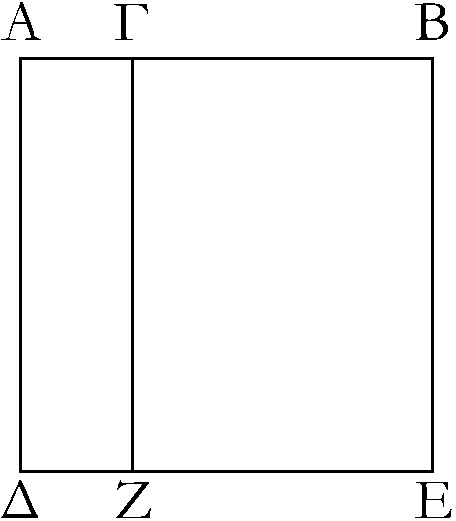
\includegraphics{Book02/fig02g.eps}}

\gr{Εὐθεῖα γὰρ ἡ ΑΒ τετμ\kern -.7pt  ήσθω, ὡξ >έτυθεν, κατὰ τὸ Γ σημεῖον; λέγω, 
<ότι τὸ ὑπὸ τῶν ΑΒ, ΒΓ περιεχόμενον ὀρθογώνιον μετὰ τοῦ ὑπὸ ΒΑ, ΑΓ περιεθομένου ὀρθογωνίου >ίσον  ἐστὶ τῶ| ἀπὸ τῆξ
ΑΒ τετραγώνῳ.}

\gr{Ἀναγεγράφθω γὰρ ἀπὸ τῆξ ΑΒ τετράγωνον τὸ ΑΔΕΒ, καὶ >ήθθω διὰ τοῦ Γ ὁποτέρᾳ τῶν ΑΔ, ΒΕ παράλληλοξ ἡ ΓΖ.}

\gr{>'Ισον δή ἐστὶ τὸ ΑΕ τοῖξ ΑΖ, ΓΕ. καί ἐστι τὸ μὲν ΑΕ τὸ ἀπὸ τῆξ ΑΒ τετράγωνον, τὸ δὲ ΑΖ τὸ ὑπὸ τῶν ΒΑ, ΑΓ περιεχόμενον ὀρθογώνιον; περιέθεται μὲν γὰρ ὑπὸ τῶν ΔΑ, ΑΓ, >ίση δὲ ἡ ΑΔ τῆ| ΑΒ; τὸ δὲ ΓΕ τὸ ὑπὸ τῶν ΑΒ, ΒΓ; >ίση γὰρ ἡ ΒΕ τῆ| ΑΒ. τὸ >άρα ὑπὸ τῶν ΒΑ, ΑΓ μετὰ τοῦ ὑπὸ τῶν ΑΒ, ΒΓ >ίσον ἐστὶ τῶ| ἀπὸ τῆξ ΑΒ τετραγώνῳ.}

\gr{Ἐὰν >άρα εὐθεῖα γραμμ\kern -.7pt  ὴ τμ\kern -.7pt  ηθῆ|, ὡξ >έτυθεν, τὸ ὑπὸ τῆξ <όληξ καὶ ἑκατέρου τῶν τμ\kern -.5pt  ημάτων περιεχόμενον ὀρθογώνιον >ίσον ἐστὶ τῶ| ἀπὸ τῆξ <όληξ τετραγώνῳ; <όπερ >έδει δεῖχαι.}}

\ParallelRText{
\begin{center}
{\large Proposition 2$^\dag$}
\end{center}

If a straight-line is cut at random,  (then) the (sum of the) rectangle(s) contained by the whole
(straight-line), and each of the pieces (of the straight-line), is equal to the square on the whole.

\epsfysize=2.2in
\centerline{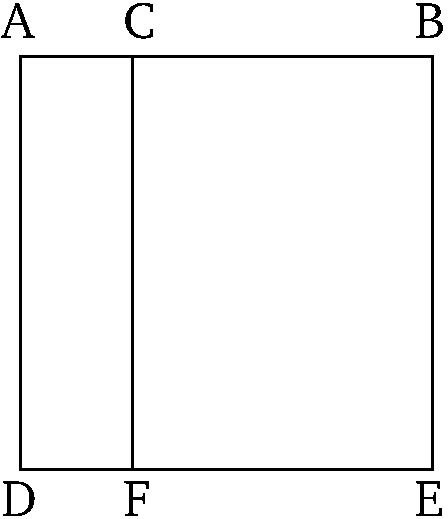
\includegraphics{Book02/fig02e.eps}}

For let the straight-line $AB$ be cut, at random, at point $C$. I say that the
rectangle contained by $AB$ and $BC$, plus the rectangle contained by 
$BA$ and $AC$, is equal to the square on $AB$.

For let the square $ADEB$ be described on $AB$ [Prop.~1.46], and
let $CF$ be drawn through $C$, parallel to either of $AD$ or $BE$ [Prop.~1.31].

So the (square) $AE$ is equal to the (rectangles) $AF$ and $CE$. And $AE$ is the square on $AB$.  And $AF$ (is) the rectangle contained by the (straight-lines) $BA$ and $AC$. For it is contained by $DA$ and $AC$, and $AD$ (is) equal to $AB$. 
And $CE$ (is) the (rectangle contained) by $AB$ and $BC$. For $BE$ (is) equal
to $AB$. Thus, the (rectangle contained) by $BA$ and $AC$, plus the
(rectangle contained) by $AB$ and $BC$, is equal to the square on $AB$.

Thus, if a straight-line is cut at random,  (then) the (sum of the) rectangle(s) contained by the whole
(straight-line), and each of the pieces (of the straight-line), is equal to the square on the whole. (Which is) the very thing it was required to show.}
\end{Parallel}
{\footnotesize \noindent$^\dag$ This proposition is a geometric version
of the algebraic identity: $a\,b+a\,c=a^{\,2}$ if $a=b+c$.}

%%%%%%
% Prop 2.3
%%%%%%
\pdfbookmark[1]{Proposition 2.3}{pdf2.3}
\begin{Parallel}{}{} 
\ParallelLText{
\begin{center}
{\large \ggn{3}.}
\end{center}\vspace*{-7pt}

\gr{Ἐὰν εὐθεῖα γραμμ\kern -.7pt  ὴ τμ\kern -.7pt  ηθῆ|, ὡξ >έτυθεν, τὸ ὑπὸ τῆξ <όληξ καὶ ἑνὸξ τῶν τμ\kern -.5pt  ημάτων περιεχόμενον ὀρθογώνιον >ίσον ἐστὶ τῶ| τε ὑπὸ τῶν τμ\kern -.3pt  ημάτων περιεθομένῳ ὀρθογωνίῳ καὶ τῶ| ἀπὸ τοῦ προειρημένου τμ\kern -.7pt  ήματοξ τετραγώνῳ.}

\epsfysize=2.in
\centerline{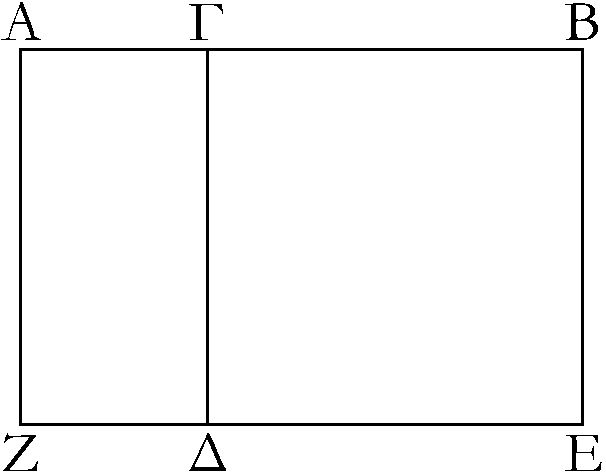
\includegraphics{Book02/fig03g.eps}}

\gr{Εὐθεῖα γὰρ ἡ ΑΒ τετμ\kern -.7pt  ήσθω, ὡξ >έτυθεν, κατὰ τὸ Γ; λέγω, <ότι
τὸ ὑπὸ τῶν ΑΒ, ΒΓ περιεχόμενον ὀρθογώνιον >ίσον ἐστὶ τῶ| τε ὑπὸ τῶν ΑΓ, ΓΒ περιεθομένῳ ὀρθογωνίῳ μετὰ τοῦ ἀπὸ τῆξ 
ΒΓ τετραγώνου.}

\gr{Ἀναγεγράφθω γὰρ ἀπὸ τῆξ ΓΒ τετράγωνον τὸ ΓΔΕΒ, καὶ διήθθω ἡ ΕΔ ἐπὶ τὸ Ζ, καὶ διὰ τοῦ Α ὁποτέρᾳ τῶν ΓΔ, ΒΕ παράλληλοξ >ήθθω ἡ ΑΖ. >ίσον δή ἐστι τὸ ΑΕ τοῖξ ΑΔ, ΓΕ; καί ἐστι τὸ μὲν ΑΕ τὸ ὑπὸ τῶν ΑΒ, ΒΓ περιεχόμενον ὀρθογώνιον; περιέθεται μὲν γὰρ ὑπὸ τῶν ΑΒ, ΒΕ, >ίση δὲ ἡ ΒΕ τῆ| ΒΓ; τὸ δὲ ΑΔ τὸ ὑπὸ τῶν ΑΓ, ΓΒ; >ίση γὰρ ἡ ΔΓ τῆ| ΓΒ; τὸ δὲ ΔΒ τὸ ἀπὸ τῆξ ΓΒ τετράγωνον; τὸ >άρα ὑπὸ τῶν ΑΒ, ΒΓ περιεχόμενον ὀρθογώνιον >ίσον ἐστὶ τῶ| ὑπὸ τῶν
ΑΓ, ΓΒ περιεθομένῳ ὀρθογωνίῳ μετὰ τοῦ ἀπὸ τῆξ ΒΓ τετραγώνου.}

\gr{Ἐὰν >άρα εὐθεῖα γραμμ\kern -.7pt  ὴ τμ\kern -.7pt  ηθῆ|, ὡξ >έτυθεν, τὸ ὑπὸ τῆξ <όληξ καὶ ἑνὸξ τῶν τμ\kern -.5pt  ημάτων περιεχόμενον ὀρθογώνιον >ίσον ἐστὶ τῶ| τε ὑπὸ τῶν τμ\kern -.3pt  ημάτων περιεθομένῳ ὀρθογωνίῳ καὶ τῶ| ἀπὸ τοῦ προειρημένου τμ\kern -.7pt  ήματοξ τετραγώνῳ; <όπερ >έδει δεῖχαι.}}

\ParallelRText{
\begin{center}
{\large Proposition 3$^\dag$}
\end{center}

If  a straight-line is cut at random, (then) the rectangle contained by the
whole (straight-line), and one of the pieces (of the straight-line),
is equal to the rectangle contained by (both of) the pieces, and the square on
the aforementioned piece.

\epsfysize=2.in
\centerline{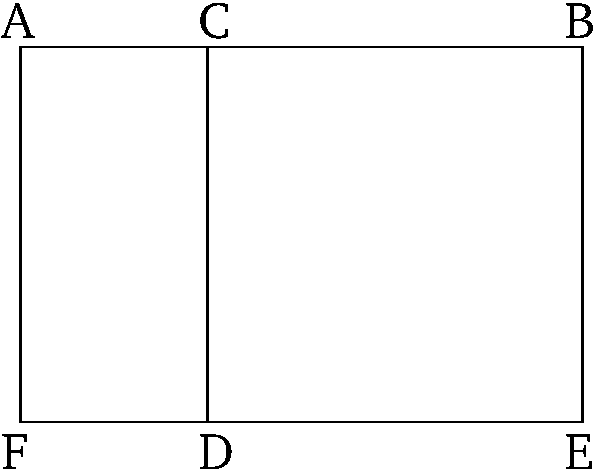
\includegraphics{Book02/fig03e.eps}}

For let the straight-line $AB$ be cut, at random, at (point) $C$.
I say that the rectangle contained by $AB$ and $BC$ is equal to the
rectangle contained by $AC$ and $CB$, plus the square on $BC$.

For let the square $CDEB$ be described on $CB$ [Prop.~1.46],
and let $ED$ be drawn through to $F$, and let $AF$ be
drawn through $A$, parallel to either of $CD$ or $BE$ [Prop.~1.31].
So the (rectangle) $AE$ is equal to the (rectangle) $AD$ and the (square) $CE$.
And $AE$ is the rectangle contained by $AB$ and $BC$.
For it is contained by $AB$ and $BE$, and $BE$ (is) equal to $BC$. And
$AD$ (is) the (rectangle contained) by $AC$ and $CB$. For $DC$
(is) equal to $CB$. And $DB$ (is) the square on $CB$. Thus, the rectangle
contained by $AB$ and $BC$ is equal to the rectangle contained by $AC$ and
$CB$, plus the square on $BC$.

Thus, if a straight-line is cut at random, (then) the rectangle contained by the
whole (straight-line),  and one of the pieces (of the straight-line),
is equal to the rectangle contained by (both of) the pieces, and the square on
the aforementioned piece. (Which is) the very thing it was required
to show.}
\end{Parallel}
{\footnotesize \noindent$^\dag$ This proposition is a geometric version
of the algebraic identity: $(a+b)\,a = a\,b + a^{\,2}$.}

%%%%%%
% Prop 2.4
%%%%%%
\pdfbookmark[1]{Proposition 2.4}{pdf2.4}
\begin{Parallel}{}{} 
\ParallelLText{
\begin{center}
{\large \ggn{4}.}
\end{center}\vspace*{-7pt}

\gr{Ἐὰν εὐθεῖα γραμμ\kern -.7pt  ὴ τμ\kern -.7pt  ηθῆ|, ὡξ >έτυθεν, τὸ ἀπὸ τῆξ <όληξ τετράγωνον >ίσον ἐστὶ τοῖξ τε ἀπὸ τῶν τμ\kern -.5pt  ημάτων τετραγώνοιξ καὶ τῶ| δὶξ ὑπὸ τῶν τμ\kern -.3pt  ημάτων περιεθομένῳ ὀρθογωνίῳ.}

\gr{Εὐθεῖα γὰρ γραμμ\kern -.7pt  ὴ ἡ ΑΒ τετμ\kern -.7pt  ήσθω, ὡξ >έτυθεν, κατὰ τὸ Γ. λέγω,
<ότι τὸ ἀπὸ τῆξ ΑΒ τετράγωνον >ίσον ἐστὶ τοῖξ τε ἀπὸ τῶν ΑΓ, ΓΒ τετραγώνοιξ καὶ τῶ| δὶξ ὑπὸ τῶν ΑΓ, ΓΒ  περιεθομένῳ ὀρθογωνίῳ.}

\gr{Ἀναγεγράφθω γὰρ ἀπὸ τῆξ ΑΒ τετράγωνον τὸ ΑΔΕΒ, καὶ ἐπεζεύθθω ἡ ΒΔ, καὶ διὰ μὲν τοῦ Γ ὁποτέρᾳ τῶν ΑΔ, ΕΒ παράλληλοξ >ήθθω ἡ ΓΖ, διὰ δὲ τοῦ Η ὁποτέρᾳ τῶν ΑΒ, ΔΕ παράλληλοξ >ήθθω ἡ 
JΚ. καὶ ἐπεὶ παράλληλόξ ἐστιν ἡ ΓΖ τῆ| ΑΔ, καὶ εἰξ α\kern -.7pt  ὐτὰξ ἐμπέπτωκεν ἡ ΒΔ, ἡ ἐκτὸξ γωνία ἡ ὑπὸ ΓΗΒ >ίση ἐστὶ τῆ| ἐντὸξ καὶ ἀπεναντίον τῆ| ὑπὸ ΑΔΒ. ἀλλ> ἡ ὑπὸ ΑΔΒ τῆ| ὑπὸ ΑΒΔ ἐστιν >ίση, ἐπεὶ καὶ πλευρὰ ἡ ΒΑ τῆ| ΑΔ ἐστιν >ίση;
καὶ ἡ ὑπὸ ΓΗΒ >άρα γωνιά τῆ| ὑπὸ ΗΒΓ ἐστιν >ίση; <ώστε καὶ πλευρὰ ἡ ΒΓ πλευρᾶ|  τῆ| ΓΗ ἐστιν >ίση;
ἀλλ> ἡ μὲν ΓΒ τῆ| ΗΚ ἐστιν >ίση, ἡ δὲ ΓΗ τῆ| ΚΒ; καὶ ἡ ΗΚ >άρα τῆ| ΚΒ ἐστιν >ίση; ἰσόπλευρον >άρα ἐστὶ  τὸ ΓΗΚΒ. λέγω δή, <ότι καὶ ὀρθογώνιον. ἐπεὶ γὰρ παράλληλόξ ἐστιν ἡ ΓΗ τῆ| ΒΚ [καὶ εἰξ α\kern -.7pt  ὐτὰξ ἐμπέπτωκεν εὐθεῖα ἡ ΓΒ], αἱ >άρα ὑπὸ ΚΒΓ, ΗΓΒ γωνίαι δύο ὀρθαῖξ εἰσιν >ίσαι. ὀρθὴ δὲ ἡ ὑπὸ ΚΒΓ; ὀρθὴ >άρα καὶ ἡ ὑπὸ ΒΓΗ; <ώστε καὶ αἱ ἀπεναντίον αἱ ὑπὸ ΓΗΚ, ΗΚΒ ὀρθαί εἰσιν. ὀρθογώνιον >άρα ἐστὶ τὸ ΓΗΚΒ; ἐδείθθη δὲ καὶ ἰσόπλευρον; τετράγωνον >άρα ἐστίν; καί ἐστιν ἀπὸ τῆξ ΓΒ. διὰ τὰ α\kern -.5pt  ὐτὰ δὴ καὶ τὸ JΖ τετράγωνόν ἐστιν; καί ἐστιν ἀπὸ τῆξ JΗ, τουτέστιν [ἀπὸ] τῆξ ΑΓ; τὰ >άρα JΖ, ΚΓ τετράγωνα ἀπὸ τῶν ΑΓ, ΓΒ εἰσιν. καὶ ἐπεὶ >ίσον ἐστὶ τὸ ΑΗ τῶ| ΗΕ, καί ἐστι τὸ ΑΗ τὸ ὑπὸ τῶν ΑΓ, ΓΒ; >ίση γὰρ ἡ ΗΓ τῆ| ΓΒ; καὶ τὸ ΗΕ >άρα >ίσον ἐστὶ τῶ| ὑπὸ ΑΓ, ΓΒ; τὰ >άρα ΑΗ, ΗΕ >ίσα ἐστὶ τῶ| δὶξ ὑπὸ τῶν ΑΓ, ΓΒ. >έστι δὲ καὶ τὰ JΖ, ΓΚ τετράγωνα ἀπὸ τῶν ΑΓ, ΓΒ; τὰ >άρα τέσσαρα τὰ JΖ, ΓΚ, ΑΗ, ΗΕ >ίσα ἐστὶ τοῖξ τε ἀπὸ τῶν ΑΓ, ΓΒ τετραγώνοιξ καὶ τῶ| δὶξ ὑπὸ τῶν ΑΓ, ΓΒ περιεθομένῳ ὀρθογωνίῳ. ἀλλὰ τὰ JΖ, ΓΚ, ΑΗ, ΗΕ <όλον ἐστὶ
τὸ ΑΔΕΒ, <ό ἐστιν ἀπὸ τῆξ ΑΒ τετράγωνον; τὸ >άρα ἀπὸ τῆξ ΑΒ τετράγωνον >ίσον ἐστὶ τοῖξ τε ἀπὸ τῶν ΑΓ, ΓΒ τετραγώνοιξ καὶ τῶ| δὶξ ὑπὸ τῶν ΑΓ, ΓΒ περιεθομένῳ ὀρθογωνίῳ.}\\~\\~\\~\\~\\

\epsfysize=2.2in
\centerline{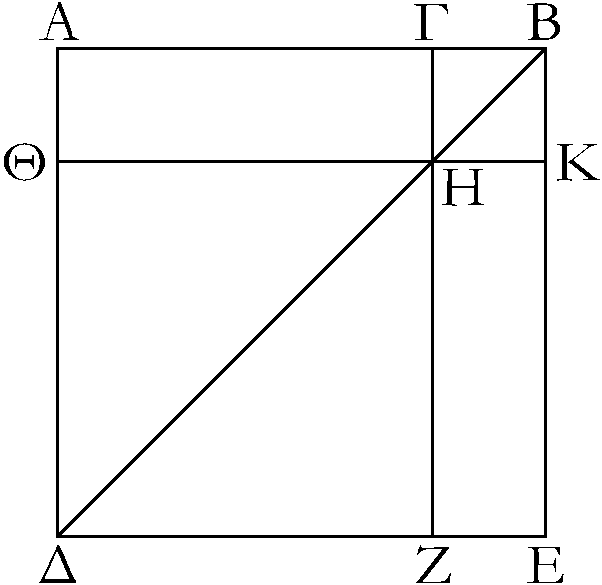
\includegraphics{Book02/fig04g.eps}}

\gr{Ἐὰν >άρα εὐθεῖα γραμμ\kern -.7pt  ὴ τμ\kern -.7pt  ηθῆ|, ὡξ >έτυθεν, τὸ ἀπὸ τῆξ <όληξ τετράγωνον >ίσον ἐστὶ τοῖξ τε ἀπὸ τῶν τμ\kern -.5pt  ημάτων τετραγώνοιξ καὶ τῶ| δὶξ ὑπὸ τῶν τμ\kern -.3pt  ημάτων περιεθομένῳ ὀρθογωνίῳ;
 <όπερ >έδει δεῖχαι.}}

\ParallelRText{
\begin{center}
{\large Proposition 4$^\dag$}
\end{center}

If a straight-line is cut at random,  (then) the square on the whole (straight-line)
is equal to the (sum of the) squares on the pieces (of the straight-line),  and twice the
rectangle contained by the pieces.

For let the straight-line $AB$ be cut, at random, at  (point) $C$. I say that the square on $AB$
is equal to the (sum of the) squares on $AC$ and $CB$, and twice the rectangle
contained by $AC$ and $CB$.

For let the square $ADEB$ be described on $AB$ [Prop.~1.46], and let $BD$ be joined, and let $CF$ be drawn through $C$, parallel to either of $AD$ or $EB$ [Prop.~1.31],
and let $HK$ be drawn through $G$, parallel to either of $AB$ or $DE$ [Prop.~1.31].
And since $CF$ is parallel to $AD$, and $BD$ has fallen across them, the external
angle $CGB$ is equal to the internal and opposite (angle) $ADB$ [Prop.~1.29].
But, $ADB$ is equal to $ABD$, since the side $BA$ is also equal to $AD$ [Prop.~1.5].
Thus, angle $CGB$ is also equal to $GBC$. So the side $BC$ is equal to the side $CG$ [Prop.~1.6]. But, $CB$ is equal to $GK$, and $CG$ to $KB$ [Prop.~1.34]. Thus, $GK$
is also equal to $KB$. Thus, $CGKB$ is equilateral. So I say that (it is) also right-angled. For since $CG$ is parallel to $BK$ [and the straight-line $CB$ has fallen across them], the angles $KBC$ and $GCB$ are thus equal to two 
right-angles
[Prop.~1.29]. But $KBC$ (is) a right-angle. Thus, 
$BCG$ (is) also a right-angle.
So the opposite (angles) $CGK$ and $GKB$ are also right-angles [Prop.~1.34]. Thus,
$CGKB$ is right-angled. And it was also shown (to be) equilateral. Thus,
it is a square. And it is on $CB$. So, for the same (reasons), $HF$ is  also a square.
And it is on $HG$, that is to say [on] $AC$ [Prop.~1.34]. Thus, the squares $HF$ and
$KC$ are on $AC$ and $CB$ (respectively). And  the (rectangle) $AG$ is
equal to the (rectangle) $GE$ [Prop.~1.43]. And $AG$ is  the (rectangle contained)
by $AC$ and $CB$. For $GC$ (is) equal to $CB$. Thus, $GE$ is also equal to the
(rectangle contained) by $AC$ and $CB$. Thus, the (rectangles)
$AG$ and $GE$ are equal to twice the (rectangle contained) by $AC$ and $CB$.
And $HF$ and $CK$ are the squares on $AC$ and $CB$ (respectively). Thus, the
four (figures) $HF$, $CK$, $AG$, and $GE$ are equal to the (sum of the) squares on $AC$ and
$BC$, and twice the rectangle contained by $AC$ and $CB$. But, the  (figures) $HF$, $CK$, $AG$, and $GE$ are (equivalent to) the whole of $ADEB$, which is the square on $AB$. 
Thus, the square on $AB$ is equal to the (sum of the) squares on $AC$ and $CB$, and twice
the rectangle contained by $AC$ and $CB$.

\epsfysize=2.2in
\centerline{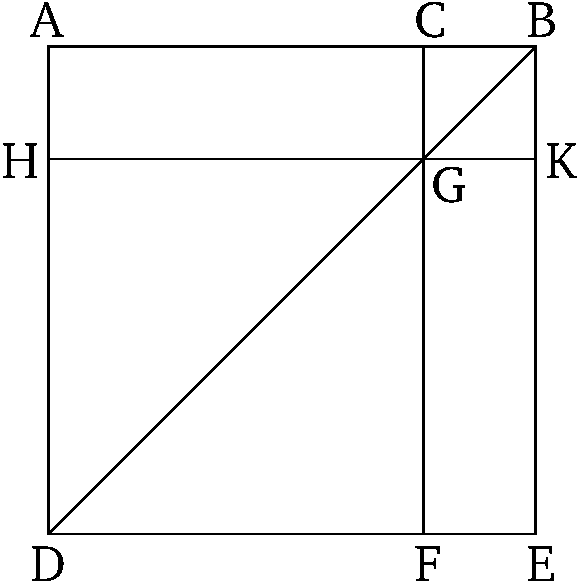
\includegraphics{Book02/fig04e.eps}}

Thus, if a straight-line is cut at random, (then) the square on the whole (straight-line) is equal to the (sum of the) squares on the pieces (of the
straight-line), and twice the
rectangle contained by the pieces. (Which is) the very thing it was required to
show.}
\end{Parallel}
{\footnotesize \noindent$^\dag$ This proposition is a geometric version
of the algebraic identity: $(a+b)^{\,2} = a^{\,2} + b^{\,2}+ 2\,a\,b$.}

%%%%%%
% Prop 2.5
%%%%%%
\pdfbookmark[1]{Proposition 2.5}{pdf2.5}
\begin{Parallel}{}{} 
\ParallelLText{
\begin{center}
{\large \ggn{5}.}
\end{center}\vspace*{-7pt}

\gr{Ἐὰν εὐθεῖα γραμμ\kern -.7pt  ὴ τμ\kern -.7pt  ηθῆ| εἰξ >ίσα καὶ >άνισα, τὸ ὑπὸ τῶν ἀνίσων τῆξ <όληξ τμ\kern -.5pt  ημάτων περιεχόμενον ὀρθογώνιον μετὰ τοῦ ἀπὸ τῆξ μεταχὺ τῶν τομῶν τετραγώνου >ίσον ἐστὶ τῶ|
ἀπὸ τῆξ ἡμισείαξ τετραγώνῳ.}\\

\epsfysize=1.8in
\centerline{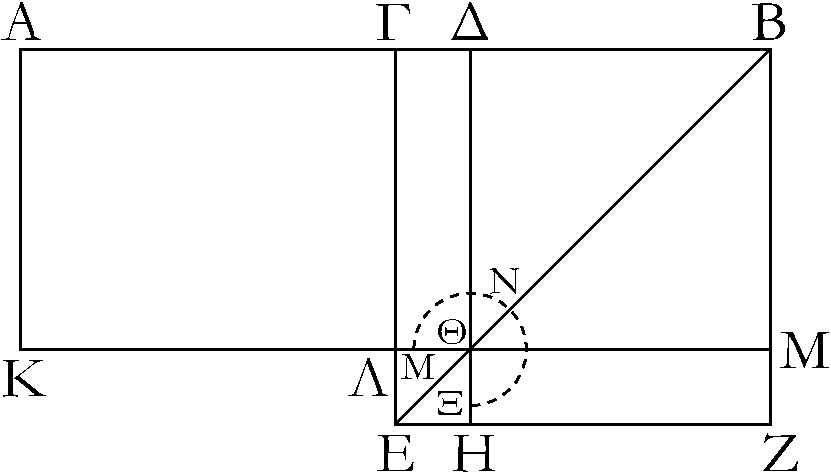
\includegraphics{Book02/fig05g.eps}}

\gr{Εὐθεῖα γάρ τιξ ἡ ΑΒ τετμ\kern -.7pt  ήσθω εἰξ μὲν >ίσα κατὰ τὸ Γ, εἰξ δὲ >άνισα κατὰ τὸ Δ; λέγω, <ότι τὸ ὑπὸ τῶν ΑΔ, ΔΒ περιεχόμενον ὀρθογώνιον μετὰ τοῦ ἀπὸ τῆξ ΓΔ τετραγώνου >ίσον ἐστὶ τῶ| ἀπὸ τῆξ ΓΒ τετραγώνῳ.}

\gr{Ἀναγεγράφθω γὰρ ἀπὸ τῆξ ΓΒ τετράγωνον τὸ ΓΕΖΒ, καὶ ἐπεζεύθθω ἡ ΒΕ, καὶ διὰ μὲν τοῦ Δ ὁποτέρᾳ τῶν ΓΕ, ΒΖ παράλληλοξ >ήθθω ἡ ΔΗ, διὰ δὲ τοῦ J ὁποτέρᾳ τῶν ΑΒ, ΕΖ παράλληλοξ πάλιν >ήθθω ἡ ΚΜ, καὶ πάλιν διὰ τοῦ Α ὁποτέρᾳ τῶν ΓΛ, ΒΜ παράλληλοξ >ήθθω ἡ ΑΚ. καὶ ἐπεὶ >ίσον ἐστὶ τὸ ΓJ παραπλήρωμα τῶ| JΖ παραπληρώματι, κοινὸν προσκείσθω τὸ ΔΜ; <όλον >άρα τὸ ΓΜ <όλῳ τῶ| ΔΖ >ίσον ἐστίν. ἀλλὰ τὸ ΓΜ τῶ| ΑΛ >ίσον ἐστίν, ἐπεὶ καὶ ἡ ΑΓ τῆ| ΓΒ ἐστιν >ίση; καὶ τὸ ΑΛ >άρα τῶ| ΔΖ >ίσον ἐστίν. κοινὸν προσκείσθω τὸ ΓJ; <όλον >άρα τὸ ΑJ τῶ| ΜΝΧ}$^{\,\dag}$ \gr{γνώμονι >ίσον ἐστίν. ἀλλὰ τὸ ΑJ τὸ ὑπὸ τῶν ΑΔ, ΔΒ ἐστιν; >ίση γὰρ ἡ ΔJ τῆ| ΔΒ; καὶ ὁ ΜΝΧ >άρα γνώμων 
>ίσοξ ἐστὶ τῶ| ὑπὸ ΑΔ, ΔΒ. κοινὸν προσκείσθω τὸ ΛΗ, <ό ἐστιν >ίσον τῶ| ἀπὸ τῆξ ΓΔ; ὁ >άρα ΜΝΧ γνώμων καὶ τὸ ΛΗ >ίσα ἐστὶ τῶ| 
ὑπὸ τῶν ΑΔ, ΔΒ περιεθομένῳ ὀρθογωνίῳ καὶ τῶ|
ἀπὸ τῆξ ΓΔ τετραγώνῳ. ἀλλὰ ὁ ΜΝΧ γνώμων 
καὶ τὸ ΛΗ  <όλον ἐστὶ τὸ ΓΕΖΒ τετράγωνον, <ό ἐστιν ἀπὸ τῆξ ΓΒ; τὸ >άρα ὑπὸ τῶν ΑΔ, ΔΒ περιεχόμενον ὀρθογώνιον μετὰ τοῦ ἀπὸ τῆξ ΓΔ τετραγώνου >ίσον ἐστὶ τῶ| ἀπὸ τῆξ ΓΒ τετραγώνῳ.}

\gr{Ἐὰν >άρα εὐθεῖα γραμμ\kern -.7pt  ὴ τμ\kern -.7pt  ηθῆ| εἰξ >ίσα καὶ >άνισα, τὸ ὑπὸ τῶν
ἀνίσων τῆξ <όληξ τμ\kern -.5pt  ημάτων περιεχόμενον ὀρθογώνιον μετὰ τοῦ ἀπὸ τῆξ μεταχὺ τῶν τομῶν τετραγώνου >ίσον ἐστὶ τῶ|
ἀπὸ τῆξ ἡμισείαξ τετραγώνῳ. <όπερ >έδει δεῖχαι.}}

\ParallelRText{
\begin{center}
{\large Proposition 5$^\ddag$}
\end{center}

If a straight-line is cut into equal and unequal (pieces, then) the rectangle contained by the
unequal pieces of the whole (straight-line), plus the square on the (difference) between the (equal and unequal)
pieces, is equal to the square on  half (of the straight-line).

\epsfysize=1.8in
\centerline{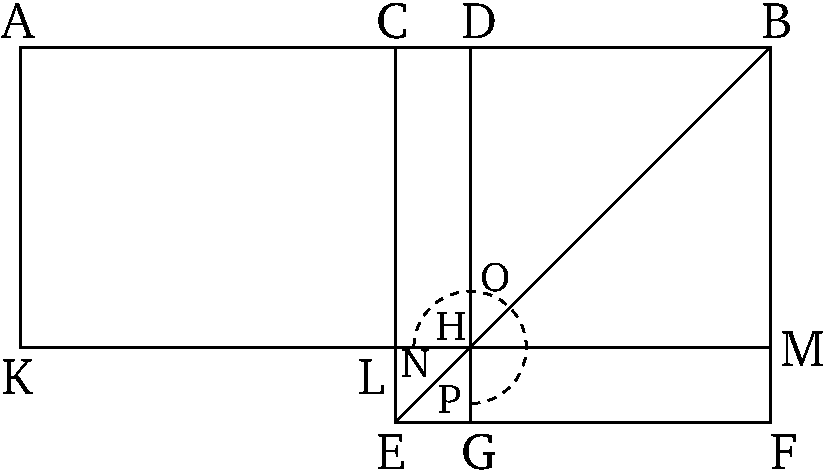
\includegraphics{Book02/fig05e.eps}}

For let any straight-line $AB$ be cut---equally at $C$, and unequally at $D$.
I say that the rectangle contained by $AD$ and $DB$, plus the square
on $CD$, is equal to the square on $CB$.

For let the square $CEFB$ be described on $CB$ [Prop.~1.46], and
let $BE$ be joined,
and let $DG$ 
be  drawn through $D$, parallel to either of $CE$ or $BF$ [Prop.~1.31], and again let $KM$
be drawn through $H$, parallel to either of $AB$ or $EF$ [Prop.~1.31], and again let
$AK$ be drawn through $A$, parallel to either of $CL$ or $BM$ [Prop.~1.31].
And since the complement $CH$ is equal to the complement $HF$ [Prop.~1.43],
let the (square) $DM$ be added to both. Thus, the whole (rectangle) $CM$ is equal to the whole (rectangle) $DF$. But, (rectangle) $CM$ is equal to (rectangle) $AL$, since $AC$ is
also equal to $CB$ [Prop.~1.36]. Thus, (rectangle) $AL$ is also equal to (rectangle) $DF$.
Let (rectangle) $CH$ be added to both. Thus, the whole (rectangle)
$AH$ is equal to the gnomon $NOP$. But,  $AH$ is the (rectangle
contained) by $AD$ and $DB$. For $DH$ (is) equal to $DB$. Thus, the
gnomon $NOP$ is also equal to the (rectangle contained) by $AD$ and $DB$. Let
$LG$, which is equal to the (square) on $CD$,  be added to both.
Thus, the gnomon $NOP$ and the (square) $LG$ are equal to the rectangle contained by
$AD$ and $DB$, and the square on $CD$. But, the gnomon $NOP$ and
the (square) $LG$ is (equivalent to) the whole square $CEFB$, which is on $CB$. Thus, the rectangle contained
by $AD$ and $DB$, plus the square on $CD$, is equal to the square on $CB$.

Thus, if a straight-line is cut into equal and unequal (pieces, then) the rectangle contained by the
unequal pieces of the whole  (straight-line), plus the square on the (difference) between the (equal and unequal)
pieces, is equal to the square on  half (of the straight-line). (Which is) the
very thing it was required to show.}
\end{Parallel}
{\footnotesize \noindent$^\dag$ Note the (presumably mistaken) double use of the label $M$ in the Greek text.\\[0.5ex]
$^\ddag$ This proposition is a geometric version
of the algebraic identity: $a\,b +[(a+b)/2-b]^{\,2} = [(a+b)/2]^{\,2}$.}

%%%%%%
% Prop 2.6
%%%%%%
\pdfbookmark[1]{Proposition 2.6}{pdf2.6}
\begin{Parallel}{}{} 
\ParallelLText{
\begin{center}
{\large \ggn{6}.}
\end{center}\vspace*{-7pt}

\gr{Ἐὰν εὐθεῖα γραμμ\kern -.7pt  ὴ τμ\kern -.7pt  ηθῆ| δίθα, προστεθῆ| δέ τιξ α\kern -.5pt  ὐτῆ| εὐθεῖα ἐπ> εὐθείαξ, τὸ ὑπὸ τῆξ <όληξ σὺν τῆ| προσκειμένῃ καὶ τῆξ προσκειμένηξ περιεχόμενον ὀρθόγώνιον μετὰ τοῦ ἀπὸ τῆξ ἡμισείαξ τετραγώνου >ίσον ἐστὶ τῶ| ἀπὸ τῆξ συγκειμένηξ >έκ τε τῆξ ἡμισείαξ καὶ τῆξ προσκειμένηξ τετραγώνῳ.}\\~\\

\epsfysize=1.8in
\centerline{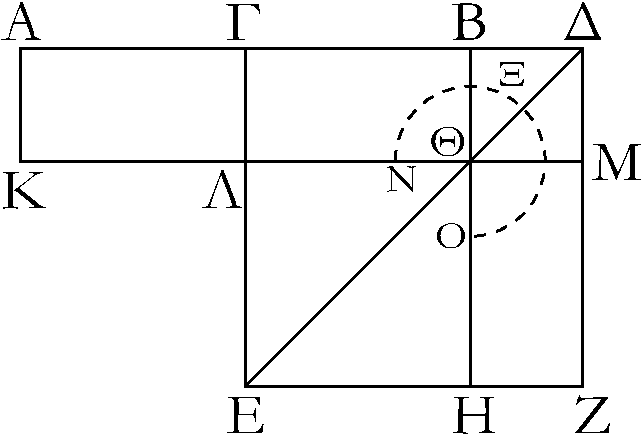
\includegraphics{Book02/fig06g.eps}}

\gr{Εὐθεῖα γάρ τιξ ἡ ΑΒ τετμ\kern -.7pt  ήσθω δίθα κατὰ τὸ Γ σημεῖον, προσκείσθω δέ τιξ α\kern -.7pt  ὐτῆ| εὐθεῖα ἐπ> εὐθείαξ ἡ ΒΔ; λέγω, <ότι τὸ ὑπὸ τῶν ΑΔ, ΔΒ περιεχόμενον ὀρθογώνιον μετὰ τοῦ ἀπὸ τῆξ ΓΒ
τετραγώνου >ίσον ἐστὶ τῶ| ἀπὸ τῆξ ΓΔ τετραγώνῳ.}

\gr{Ἀναγεγράφθω γὰρ ἀπὸ τῆξ ΓΔ τετράγωνον τὸ ΓΕΖΔ, καὶ ἐπεζεύθθω
ἡ ΔΕ, καὶ διὰ μὲν τοῦ Β σημείου ὁποτέρᾳ τῶν ΕΓ, ΔΖ παράλληλοξ >ήθθω ἡ ΒΗ, διὰ δὲ τοῦ J σημείου ὁποτέρᾳ τῶν ΑΒ, ΕΖ παράλληλοξ >ήθθω ἡ ΚΜ, καὶ >έτι διὰ τοῦ Α ὁποτέρᾳ τῶν ΓΛ, ΔΜ παράλληλοξ >ήθθω ἡ ΑΚ.}

\gr{Ἐπεὶ ο>ῦν >ίση ἐστὶν  ἡ ΑΓ τῆ| ΓΒ, >ίσον ἐστὶ καὶ τὸ ΑΛ τῶ| ΓJ. ἀλλὰ τὸ ΓJ τῶ| JΖ >ίσον ἐστίν. καὶ τὸ ΑΛ >άρα τῶ| JΖ ἐστιν >ίσον.
κοινὸν προσκείσθω τὸ ΓΜ; <όλον >άρα τὸ ΑΜ τῶ| ΝΧΟ γνώμονί ἐστιν >ίσον. ἀλλὰ τὸ ΑΜ ἐστι τὸ ὑπὸ τῶν ΑΔ, ΔΒ; >ίση γάρ ἐστιν ἡ ΔΜ τῆ| ΔΒ; καὶ ὁ ΝΧΟ >άρα γνώμων >ίσοξ ἐστὶ τῶ| ὑπὸ τῶν ΑΔ, ΔΒ
[περιεθομένῳ ὀρθογωνίῳ]. κοινὸν προσκείσθω τὸ ΛΗ, <ό ἐστιν >ίσον τῶ| ἀπὸ τῆξ ΒΓ τετραγώνῳ; τὸ >άρα ὑπὸ τῶν
ΑΔ, ΔΒ περιεχόμενον ὀρθογώνιον μετὰ τοῦ ἀπὸ τῆξ ΓΒ τετραγώνου 
>ίσον ἐστὶ τῶ| ΝΧΟ γνώμονι καὶ τῶ| ΛΗ. ἀλλὰ ὁ ΝΧΟ γνώμων καὶ τὸ ΛΗ <όλον ἐστὶ τὸ ΓΕΖΔ τετράγωνον, <ό ἐστιν ἀπὸ τῆξ ΓΔ; τὸ >άρα ὑπὸ τῶν ΑΔ, ΔΒ περιεχόμενον ὀρθογώνιον μετὰ τοῦ ἀπὸ τῆξ ΓΒ τετραγώνου >ίσον ἐστὶ τῶ| ἀπὸ τῆξ ΓΔ τετραγώνῳ.}

\gr{Ἐὰν >άρα εὐθεῖα γραμμ\kern -.7pt  ὴ τμ\kern -.7pt  ηθῆ| δίθα, προστεθῆ| δέ τιξ α\kern -.5pt  ὐτῆ| εὐθεῖα ἐπ> εὐθείαξ, τὸ ὑπὸ τῆξ <όληξ σὺν τῆ| προσκειμένῃ καὶ τῆξ προσκειμένηξ περιεχόμενον ὀρθόγώνιον μετὰ τοῦ ἀπὸ τῆξ ἡμισείαξ τετραγώνου >ίσον ἐστὶ τῶ| ἀπὸ τῆξ συγκειμένηξ >έκ τε τῆξ ἡμισείαξ καὶ τῆξ προσκειμένηξ τετραγώνῳ; <όπερ >έδει δεῖχαι.}}

\ParallelRText{
\begin{center}
{\large Proposition 6$^\dag$}
\end{center}

If a straight-line is cut in half, and any straight-line added to it straight-on,
(then) the rectangle contained by the whole (straight-line) with the (straight-line) having being added, and the (straight-line) having being added,   plus the square on  half (of the original straight-line), is equal to the square on the
sum of  half  (of the original straight-line) and the (straight-line) having been added.

\epsfysize=1.8in
\centerline{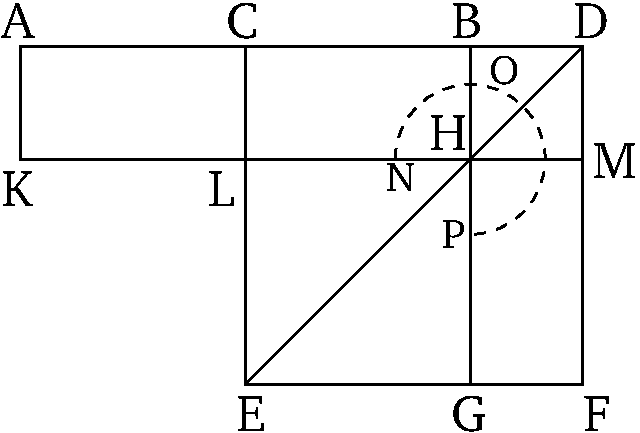
\includegraphics{Book02/fig06e.eps}}

For let any straight-line $AB$ be cut in half at point $C$, and let any
straight-line $BD$ be added to it straight-on. I say that the rectangle
contained by $AD$ and $DB$, plus the square on $CB$, is equal to the square on
$CD$.

For let the square $CEFD$ be described on $CD$ [Prop.~1.46], and let $DE$ be
joined, and let $BG$ be drawn through point $B$, parallel to either of $EC$
or $DF$ [Prop.~1.31], and let $KM$ be drawn through point $H$, parallel
to either of $AB$ or $EF$ [Prop.~1.31], and finally let $AK$ be drawn
through $A$, parallel to either of $CL$ or $DM$ [Prop.~1.31].

Therefore, since $AC$ is equal to $CB$, (rectangle) $AL$ is also equal to (rectangle) $CH$ [Prop.~1.36]. But, (rectangle) $CH$ is equal to (rectangle) $HF$ [Prop.~1.43]. Thus, (rectangle) $AL$ is also equal to (rectangle) $HF$. Let (rectangle) $CM$ 
be  added to both. Thus, the whole (rectangle) $AM$ is equal to the gnomon $NOP$.
But, $AM$ is  the (rectangle contained) by $AD$ and $DB$. For
$DM$ is equal to $DB$. Thus, gnomon $NOP$ is also equal to the
[rectangle contained] by $AD$ and $DB$.
Let $LG$, which is equal to the square on $BC$, be added to both.
Thus, the rectangle contained by $AD$ and $DB$, plus the square on $CB$, is equal
to the gnomon $NOP$ and the (square) $LG$. But the gnomon $NOP$ and 
the (square) $LG$ is (equivalent to) the whole square $CEFD$, which is on  $CD$. Thus, the rectangle
contained by $AD$ and $DB$, plus the square on $CB$, is equal to the square on $CD$.

Thus, if a straight-line is cut in half, and any straight-line added to it straight-on,
(then) the rectangle contained by the whole (straight-line) with the (straight-line) having being added, and the (straight-line) having being added,   plus the square on  half (of the original straight-line), is equal to the square on the
sum of  half  (of the original straight-line) and the (straight-line) having been added. (Which is) the very thing it was required to show.}
\end{Parallel}
{\footnotesize \noindent$^\dag$ This proposition is a geometric version
of the algebraic identity: $(2\,a+b)\,b + a^{\,2} = (a+b)^{\,2}$.}

%%%%%%
% Prop 2.7
%%%%%%
\pdfbookmark[1]{Proposition 2.7}{pdf2.7}
\begin{Parallel}{}{} 
\ParallelLText{
\begin{center}
{\large \ggn{7}.}
\end{center}\vspace*{-7pt}

\gr{Ἐὰν εὐθεῖα γραμμ\kern -.7pt  ὴ  τμ\kern -.7pt  ηθῆ|, ὡξ >έτυθεν, τὸ ἀπὸ τῆξ <όληξ καὶ τὸ ἀφ> ἑνὸξ τῶν τμ\kern -.5pt  ημάτων τὰ συναμφότερα τετράγωνα >ίσα ἐστὶ τῶ| τε δὶξ ὑπὸ τῆξ <όληξ καὶ τοῦ εἰρημένου τμ\kern -.3pt  ήματοξ περιεθομένῳ ὀρθογωνίῳ καὶ τῶ| ἀπὸ τοῦ λοιποῦ τμ\kern -.7pt  ήματοξ τετραγώνῳ.}

\epsfysize=2.2in
\centerline{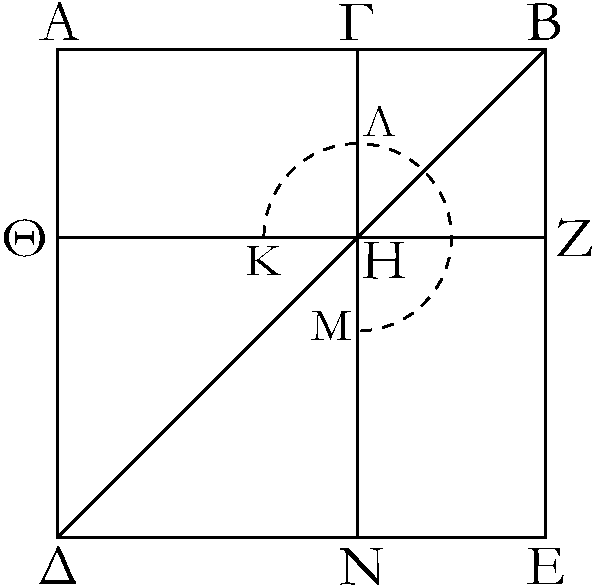
\includegraphics{Book02/fig07g.eps}}

\gr{Εὐθεῖα γάρ τιξ ἡ ΑΒ τετμ\kern -.7pt  ήσθω, ὡξ >έτυθεν, κατὰ τὸ Γ σημεῖον; λέγω, <ότι τὰ ἀπὸ τῶν ΑΒ, ΒΓ τετράγωνα >ίσα ἐστὶ τῶ| τε δὶξ ὑπὸ τῶν
ΑΒ, ΒΓ περιεθομένῳ ὀρθογωνίῳ καὶ τῶ| ἀπὸ τῆξ ΓΑ τετραγώνῳ.}

\gr{Ἀναγεγράφθω γὰρ ἀπὸ τῆξ ΑΒ τετράγωνον τὸ ΑΔΕΒ; καὶ καταγεγράφθω τὸ σθῆμα.}

\gr{Ἐπεὶ ο>ῦν >ίσον ἐστὶ τὸ ΑΗ τῶ| ΗΕ, κοινὸν προσκείσθω τὸ ΓΖ; <όλον >άρα τὸ ΑΖ <όλῳ τῶ| ΓΕ >ίσον ἐστίν; τὰ >άρα ΑΖ, ΓΕ διπλάσιά ἐστι τοῦ ΑΖ. ἀλλὰ τὰ ΑΖ, ΓΕ ὁ ΚΛΜ ἐστι γνώμων καὶ τὸ ΓΖ
τετράγωνον; ὁ ΚΛΜ >άρα γνώμων καὶ τὸ ΓΖ διπλάσιά ἐστι τοῦ ΑΖ. >έστι δὲ τοῦ ΑΖ διπλάσιον καὶ τὸ δὶξ ὑπὸ τῶν ΑΒ, ΒΓ;
>ίση γὰρ ἡ ΒΖ τῆ| ΒΓ; ὁ >άρα ΚΛΜ γνώμων καὶ τὸ ΓΖ τετράγωνον
>ίσον  ἐστὶ τῶ| δὶξ ὑπὸ τῶν ΑΒ, ΒΓ.
 κοινὸν προσκείσθω τὸ ΔΗ, <ό ἐστιν ἀπὸ τῆξ ΑΓ τετράγωνον; ὁ >άρα ΚΛΜ
γνώμων καὶ τὰ ΒΗ, ΗΔ τετράγωνα >ίσα ἐστὶ τῶ| τε δὶξ ὑπὸ τῶν ΑΒ, ΒΓ περιεθομένῳ ὀρθογωνίῳ  καὶ τῶ| ἀπὸ τῆξ ΑΓ τετραγώνῳ.
ἀλλὰ ὁ ΚΛΜ γνώμων καὶ τὰ ΒΗ, ΗΔ τετράγωνα <όλον ἐστὶ τὸ ΑΔΕΒ καὶ τὸ ΓΖ,  <ά ἐστιν ἀπὸ τῶν ΑΒ, ΒΓ
 τετράγωνα; τὰ >άρα ἀπὸ τῶν ΑΒ, ΒΓ 
 τετράγωνα >ίσα ἐστὶ τῶ| [τε] δὶξ ὑπὸ τῶν ΑΒ, ΒΓ 
 περιεθομένῳ ὀρθογωνίῳ μετὰ τοῦ ἀπὸ τῆξ ΑΓ τετραγώνου.}
 
 \gr{Ἐὰν >άρα εὐθεῖα γραμμ\kern -.7pt  ὴ  τμ\kern -.7pt  ηθῆ|, ὡξ >έτυθεν, τὸ ἀπὸ τῆξ <όληξ καὶ τὸ ἀφ> ἑνὸξ τῶν τμ\kern -.5pt  ημάτων τὰ συναμφότερα τετράγωνα >ίσα ἐστὶ τῶ| τε δὶξ ὑπὸ τῆξ <όληξ καὶ τοῦ εἰρημένου τμ\kern -.3pt  ήματοξ περιεθομένῳ ὀρθογωνίῳ καὶ τῶ| ἀπὸ τοῦ λοιποῦ τμ\kern -.7pt  ήματοξ τετραγώνῳ; <όπερ >έδει δεῖχαι.}}

\ParallelRText{
\begin{center}
{\large Proposition 7$^\dag$}
\end{center}

If a straight-line is cut at random, (then) the sum of the squares on the
whole (straight-line), and one of the pieces (of the straight-line),  is equal to twice the rectangle
contained by the whole, and the said piece, and the square
on the remaining piece.

\epsfysize=2.2in
\centerline{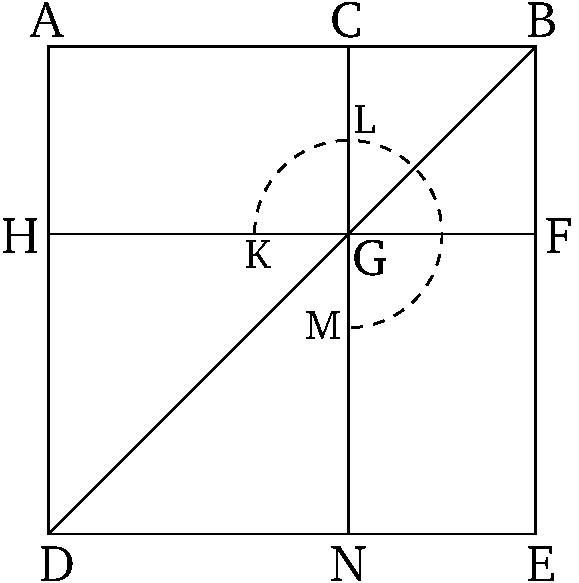
\includegraphics{Book02/fig07e.eps}}

For let any straight-line $AB$ be cut, at random, at point $C$.
I say that the (sum of the) squares on $AB$ and $BC$ is equal to
twice the rectangle contained by $AB$ and $BC$, and the square on $CA$.

For let the square $ADEB$ be described on $AB$ [Prop.~1.46], and let the (rest of)
the figure be  drawn.

Therefore, since (rectangle) $AG$ is equal to (rectangle) $GE$ [Prop.~1.43],
let the (square) $CF$ be added to both. Thus, the
whole (rectangle) $AF$ is equal to the whole (rectangle) $CE$.
Thus, (rectangle) $AF$ plus (rectangle) $CE$ is double (rectangle) $AF$.
But, (rectangle) $AF$ plus (rectangle) $CE$ is the gnomon $KLM$, and the
square  $CF$. Thus, the gnomon $KLM$, and the square $CF$, is double the (rectangle)
$AF$.
But double the (rectangle) $AF$ is also twice the (rectangle contained)
by $AB$ and $BC$. For $BF$ (is) equal to $BC$. Thus, the gnomon $KLM$, and
the square $CF$, are equal to twice the (rectangle contained) by $AB$ and $BC$.
Let $DG$, which is the square on $AC$, be added to both.
Thus, the gnomon $KLM$, and the squares $BG$ and $GD$, are equal to
twice the rectangle contained by $AB$ and $BC$, and the square on $AC$.
But, the gnomon $KLM$ and the squares $BG$ and $GD$ is (equivalent to)
the whole of
$ADEB$ and $CF$, which are the squares on $AB$ and $BC$ (respectively).
Thus, the (sum of the) squares on $AB$ and $BC$ is equal to
twice the rectangle contained by $AB$ and $BC$, and the square on $AC$.

Thus, if a straight-line is cut at random, (then) the sum of the squares on the
whole (straight-line), and one of the pieces (of the straight-line), is equal to twice the rectangle
contained by the whole,  and the said piece, and the square
on the remaining piece. (Which is) the very thing it was required to show.}
\end{Parallel}
{\footnotesize \noindent$^\dag$ This proposition is a geometric version
of the algebraic identity: $(a+b)^{\,2}+a^2 =2\,(a+b)\,a+b^{\,2}$.}

%%%%%%
% Prop 2.8
%%%%%%
\pdfbookmark[1]{Proposition 2.8}{pdf2.8}
\begin{Parallel}{}{} 
\ParallelLText{
\begin{center}
{\large \ggn{8}.}
\end{center}\vspace*{-7pt}

\gr{Ἐὰν εὐθεῖα γραμμ\kern -.7pt  ὴ τμ\kern -.7pt  ηθῆ|, ὡξ >έτυθεν, τὸ τετράκιξ ὑπὸ τῆξ <όληξ καὶ ἑνὸξ τῶν τμ\kern -.5pt  ημάτων περιεχόμενον ὀρθογώνιον μετὰ τοῦ ἀπὸ τοῦ λοιποῦ τμ\kern -.3pt  ήματοξ τετραγώνου >ίσον ἐστὶ τῶ| ἀπό τε τῆξ <όληξ καὶ τοῦ εἰρημένου τμ\kern -.7pt  ήματοξ ὡξ ἀπὸ μιᾶξ ἀναγραφέντι τετραγώνῳ.}

\gr{Εὐθεῖα γάρ τιξ ἡ ΑΒ τετμ\kern -.7pt  ήσθω, ὡξ >έτυθεν, κατὰ τὸ Γ σημεῖον; λέγω, <ότι τὸ τετράκιξ ὑπὸ τῶν ΑΒ, ΒΓ περιεχόμενον ὀρθογώνιον μετὰ τοῦ ἀπὸ τῆξ ΑΓ τετραγώνου >ίσον ἐστὶ τῶ| ἀπὸ τῆξ ΑΒ, ΒΓ ὡξ ἀπὸ μιᾶξ ἀναγραφέντι τετραγώνῳ.}

\gr{Ἐκβεβλήσθω γὰρ ἐπ> εὐθείαξ [τῆ| ΑΒ εὐθεῖα] ἡ ΒΔ, καὶ κείσθω τῆ| ΓΒ >ίση ἡ ΒΔ, καὶ ἀναγεγράφθω ἀπὸ τῆξ ΑΔ τετράγωνον τὸ ΑΕΖΔ, καὶ καταγεγράφθω διπλοῦν τὸ σθῆμα.}\\

\epsfysize=2.5in
\centerline{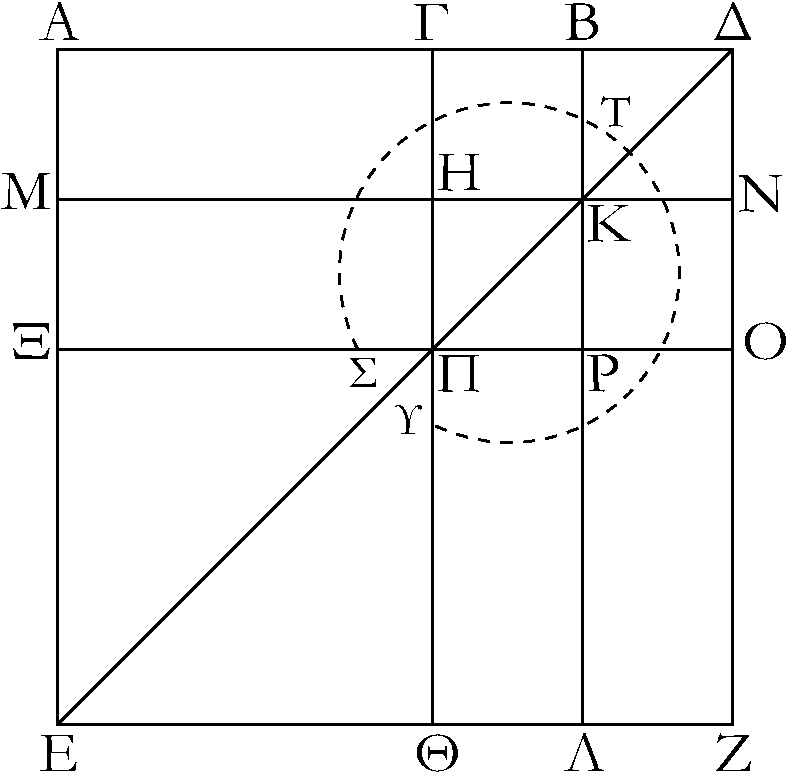
\includegraphics{Book02/fig08g.eps}}

\gr{Ἐπεὶ ο>ῦν >ίση ἐστὶν ἡ ΓΒ τῆ| ΒΔ, ἀλλὰ ἡ μὲν ΓΒ τῆ| ΗΚ ἐστιν >ίση, ἡ δὲ ΒΔ τῆ| ΚΝ, καὶ ἡ ΗΚ >άρα τῆ| ΚΝ ἐστιν >ίση. διὰ τὰ α\kern -.7pt  ὐτὰ δὴ καὶ ἡ ΠΡ τῆ| ΡΟ ἐστιν >ίση. καὶ ἐπεὶ >ίση ἐστὶν ἡ ΒΓ
τὴ| ΒΔ, ἡ δὲ ΗΚ τῆ| ΚΝ, >ίσον >άρα ἐστὶ καὶ τὸ μὲν ΓΚ τῶ| ΚΔ, τὸ δὲ ΗΡ τῶ| ΡΝ. ἀλλὰ τὸ ΓΚ τῶ| ΡΝ ἐστιν >ίσον; παραπληρώματα γὰρ τοῦ ΓΟ παραλληλογράμμου; καὶ τὸ ΚΔ >άρα τῶ| ΗΡ >ίσον ἐστίν; τὰ τέσσαρα >άρα τὰ ΔΚ, ΓΚ, ΗΡ, ΡΝ >ίσα ἀλλήλοιξ ἐστίν. τὰ τέσσαρα >άρα τετραπλάσιά ἐστι τοῦ ΓΚ. πάλιν ἐπεὶ >ίση ἐστὶν ἡ ΓΒ τῆ| ΒΔ, ἀλλὰ ἡ μὲν ΒΔ τῆ| ΒΚ, τουτέστι τῆ| ΓΗ >ίση, ἡ δὲ ΓΒ τῆ| ΗΚ, τουτέστι
τῆ| ΗΠ, ἐστιν >ίση, καὶ ἡ ΓΗ >άρα τῆ| ΗΠ >ίση ἐστίν. καὶ ἐπεὶ >ίση
ἐστὶν ἡ μὲν ΓΗ τῆ| ΗΠ, ἡ δὲ ΠΡ τῆ| ΡΟ, >ίσον ἐστὶ καὶ τὸ μὲν ΑΗ τῶ| ΜΠ, τὸ δὲ ΠΛ τῶ| ΡΖ. ἀλλὰ τὸ ΜΠ τῶ| ΠΛ ἐστιν >ίσον;
παραπληρώματα γὰρ τοῦ ΜΛ παραλληλογράμμου; καὶ τὸ ΑΗ >άρα τῶ| ΡΖ
>ίσον ἐστίν; τὰ τέσσαρα >άρα τὰ ΑΗ, ΜΠ, ΠΛ, ΡΖ
>ίσα ἀλλήλοιξ ἐστίν; τὰ τέσσαρα >άρα τοῦ ΑΗ ἐστι τετραπλάσια. ἐδείθθη
δὲ καὶ τὰ τέσσαρα τὰ ΓΚ, ΚΔ, ΗΡ, ΡΝ τοῦ ΓΚ τετραπλάσια; τὰ >άρα ὀκτώ,
<ὰ περιέθει τὸν ΣΤΥ γνώμονα, τετραπλάσιά ἐστι τοῦ ΑΚ. καὶ ἐπεὶ τὸ ΑΚ τὸ ὑπὸ τῶν ΑΒ, ΒΔ ἐστιν; >ίση γὰρ ἡ ΒΚ τῆ| ΒΔ; τὸ >άρα τετράκιξ ὑπὸ τῶν ΑΒ, ΒΔ τετραπλάσιόν ἐστι τοῦ ΑΚ. ἐδείθθη δὲ τοῦ
ΑΚ τετραπλάσιοξ καὶ ὁ ΣΤΥ γνώμων; τὸ >άρα  τετράκιξ ὑπὸ τῶν
ΑΒ, ΒΔ >ίσον ἐστὶ τῶ| ΣΤΥ γνώμονι. κοινὸν προσκείσθω τὸ ΧJ, <ό ἐστιν >ίσον τῶ| ἀπὸ τῆξ ΑΓ τετραγώνῳ; τὸ  >άρα τετράκιξ  ὑπὸ τῶν  ΑΒ,  ΒΔ περιεχόμενον ὀρθογώνιον μετὰ τοῦ ἀπὸ ΑΓ τετραγώνου >ίσον ἐστὶ τῶ| ΣΤΥ γνώμονι καὶ τῶ| ΧJ. ἀλλὰ ὁ ΣΤΥ γνώμων
καὶ τὸ ΧJ <όλον ἐστὶ τὸ ΑΕΖΔ τετράγωνον, <ό ἐστιν ἀπὸ τῆξ ΑΔ; τὸ >άρα τετράκιξ ὑπὸ τῶν ΑΒ, ΒΔ μετὰ τοῦ ἀπὸ ΑΓ >ίσον ἐστὶ τῶ| ἀπὸ ΑΔ τετραγώνῳ; >ίση δὲ ἡ ΒΔ τῆ| ΒΓ. τὸ >άρα τετράκιξ ὑπὸ τῶν ΑΒ, ΒΓ 
περιεχόμενον ὀρθογώνιον μετὰ τοῦ ἀπὸ ΑΓ τετραγώνου >ίσον ἐστὶ τῶ| ἀπὸ τῆξ ΑΔ, τουτέστι τῶ| ἀπὸ τῆξ ΑΒ καὶ ΒΓ ὡξ ἀπὸ μιᾶξ ἀναγραφέντι τετραγώνῳ.}

\gr{Ἐὰν >άρα  εὐθεῖα γραμμ\kern -.7pt  ὴ τμ\kern -.7pt  ηθῆ|, ὡξ >έτυθεν, τὸ τετράκιξ ὑπὸ τῆξ <όληξ καὶ ἑνὸξ τῶν τμ\kern -.5pt  ημάτων περιεχόμενον ὀρθογώ\-νιον μετὰ τοῦ ἀπὸ τοῦ λοιποῦ τμ\kern -.3pt  ήματοξ τετραγώνου >ίσου ἐστὶ τῶ| ἀπό τε τῆξ <όληξ καὶ τοῦ εἰρημένου τμ\kern -.7pt  ήματοξ ὡξ ἀπὸ μιᾶξ ἀναγραφέντι τετραγώνῳ;  <όπερ >έδει δεῖχαι.}}

\ParallelRText{
\begin{center}
{\large Proposition 8$^\dag$}
\end{center}

If a straight-line is cut at random, (then) four times the rectangle contained
by the whole (straight-line), and one of the pieces (of the straight-line), plus the square on the remaining piece,
is equal to the square described on the whole and the former piece, as
on one (complete straight-line).

For let any straight-line $AB$ be cut, at random, at point $C$. I say that
four times the rectangle contained by $AB$ and $BC$, plus the square on $AC$,
is equal to the square described on $AB$ and $BC$,  as on one (complete straight-line).

For let $BD$ be produced in a straight-line [with the straight-line $AB$],
and let $BD$ be made equal to $CB$ [Prop.~1.3], and let the square $AEFD$
be described on $AD$ [Prop.~1.46], and let the (rest of the) figure
be drawn double.

\epsfysize=2.5in
\centerline{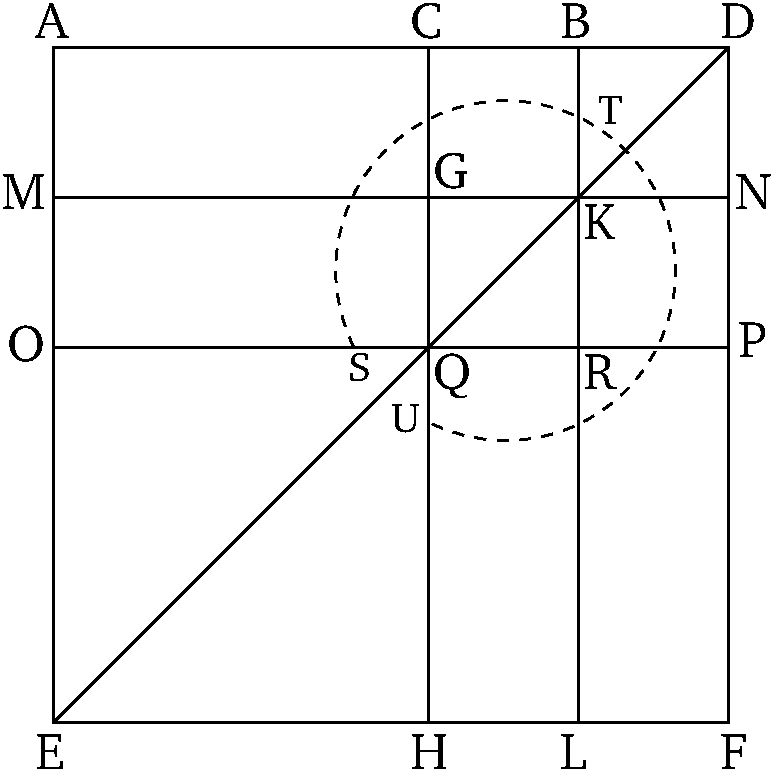
\includegraphics{Book02/fig08e.eps}}

Therefore, since $CB$ is equal to $BD$, but $CB$ is equal to $GK$ [Prop.~1.34], and $BD$ to
$KN$ [Prop.~1.34], $GK$ is thus also equal to $KN$. So, for the same (reasons), $QR$ is equal
to $RP$. And since $BC$ is equal to $BD$, and $GK$ to $KN$, (square) $CK$ is thus
also equal to (square) $KD$, and (square) $GR$ to (square) $RN$ [Prop.~1.36]. But,
(square) $CK$ is equal to (square) $RN$. For (they are) complements
in the parallelogram $CP$ [Prop.~1.43]. Thus, (square) $KD$ is also equal
to (square) $GR$. Thus, the four (squares)
$DK$, $CK$, $GR$, and $RN$ are equal to one another. Thus, the four (taken
together) are quadruple (square) $CK$. Again, since $CB$ is equal to $BD$, but
$BD$ (is) equal to $BK$---that is to say, $CG$---and $CB$ is equal to $GK$---that is
to say, $GQ$---$CG$ is thus also equal to $GQ$. And since
$CG$ is equal to $GQ$, and $QR$ to $RP$, (rectangle) $AG$ is also equal to
(rectangle) $MQ$, and (rectangle) $QL$ to (rectangle) $RF$ [Prop.~1.36]. But, (rectangle)
$MQ$ is equal to (rectangle) $QL$. For (they are) complements in the parallelogram $ML$ [Prop.~1.43]. Thus, 
(rectangle) $AG$ is also equal  to (rectangle) $RF$. Thus, the four (rectangles) $AG$, $MQ$, $QL$, and $RF$ are equal
to one another. Thus, the four (taken together)
 are quadruple (rectangle)
$AG$. And it was also shown that the four (squares)
$CK$, $KD$, $GR$, and $RN$ (taken together are) quadruple (square) $CK$. 
Thus, the eight (figures taken together), which comprise the gnomon $STU$,
are quadruple (rectangle) $AK$. And since $AK$ is the (rectangle contained)
by $AB$ and $BD$, for $BK$ (is) equal to $BD$, four times the (rectangle contained)
by $AB$ and $BD$ is quadruple (rectangle) $AK$. But the gnomon $STU$ was also shown (to be equal to) quadruple (rectangle)
$AK$. Thus, four times the
(rectangle contained) by $AB$ and $BD$ is equal to the gnomon $STU$. 
Let $OH$, which is equal to the square on $AC$,  be added to both.  
Thus, four times  the
rectangle contained by $AB$ and $BD$, plus the square on $AC$, is equal to
the gnomon $STU$, and the (square) $OH$. But, the  gnomon $STU$
and the (square) $OH$ is (equivalent to) the whole square $AEFD$, which is on
$AD$. Thus, four times the (rectangle contained) by $AB$ and $BD$, plus
the (square) on $AC$, is equal to the square on $AD$.
And $BD$ (is) equal to $BC$. Thus, four times the rectangle contained by $AB$ and $BC$, plus the square on $AC$, is equal to the (square) on $AD$, that is to
say the square described on $AB$ and $BC$,  as on one (complete straight-line).

Thus, if a straight-line is cut at random, (then) four times the rectangle contained
by the whole (straight-line), and one of the pieces (of the straight-line), plus the square on the remaining piece,
is equal to  the square described on the whole and the former piece, as
on one (complete straight-line). (Which is) the very thing it was required to show.}
\end{Parallel}
{\footnotesize \noindent$^\dag$ This proposition is a geometric version
of the algebraic identity: $4\,(a+b)\,a+b^{\,2} = \left[(a+b)+a\right]^{\,2}$.}

%%%%%%
% Prop 2.9
%%%%%%
\pdfbookmark[1]{Proposition 2.9}{pdf2.9}
\begin{Parallel}{}{} 
\ParallelLText{
\begin{center}
{\large \ggn{9}.}
\end{center}\vspace*{-7pt}

\gr{Ἐὰν εὐθεῖα γραμμ\kern -.7pt  ὴ τμ\kern -.7pt  ηθῆ| εἰξ >ίσα καὶ >άνισα, τὰ ἀπὸ τῶν ἀνίσων τῆξ <όληξ τμ\kern -.5pt  ημάτων τετράγωνα διπλάσιά ἐστι τοῦ τε ἀπὸ τῆξ ἡμισείαξ καὶ τοῦ ἀπὸ τῆξ μεταχὺ τῶν τομῶν τετραγώνου.}

\gr{Εὐθεῖα γάρ τιξ ἡ ΑΒ τετμ\kern -.7pt  ήσθω εἰξ μὲν >ίσα κατὰ τὸ Γ, εἱξ δὲ >άνισα κατὰ τὸ Δ; λέγω, <ότι τὰ ἀπὸ τῶν ΑΔ, ΔΒ τετράγωνα διπλάσιά ἐστι τῶν ἀπὸ τῶν ΑΓ, ΓΔ τετραγώνων.}

\gr{>'Ηθθω γὰρ ἀπὸ τοῦ Γ τῆ| ΑΒ πρὸξ ὀρθὰξ ἡ ΓΕ, καὶ κείσθω >ίση ἑκατέρᾳ τῶν ΑΓ, ΓΒ, καὶ ἐπεζεύθθωσαν αἱ ΕΑ, ΕΒ, καὶ διὰ μὲν τοῦ Δ τῆ| ΕΓ παράλληλοξ >ήθθω ἡ ΔΖ, διὰ δὲ τοῦ Ζ τῆ| ΑΒ ἡ ΖΗ, καὶ ἐπεζεύθθω ἡ ΑΖ. καὶ ἐπεὶ >ίση ἐστὶν ἡ ΑΓ τῆ| ΓΕ, >ίση ἐστὶ καὶ ἡ ὑπὸ ΕΑΓ γωνία τῆ| ὑπὸ ΑΕΓ. καὶ ἐπεὶ ὀρθή ἐστιν ἡ πρὸξ τῶ| Γ, λοιπαὶ >άρα αἱ ὑπὸ ΕΑΓ, ΑΕΓ μιᾶ| ὀρθῆ| >ίσαι εἰσίν;
καί εἰσιν >ίσαι; ἡμίσεια >άρα ὀρθῆξ ἐστιν ἑκατέρα τῶν ὑπὸ ΓΕΑ,
ΓΑΕ. δὶα τὰ α\kern -.7pt  ὐτὰ δὴ καὶ ἑκατέρα τῶν ὑπὸ ΓΕΒ, ΕΒΓ ἡμίσειά ἐστιν ὀρθῆξ; <όλη >άρα ἡ ὑπὸ ΑΕΒ ὀρθή ἐστιν. καὶ ἐπεὶ ἡ ὑπὸ ΗΕΖ ἡμίσειά ἐστιν ὀρθῆξ, ὀρθὴ δὲ ἡ ὑπὸ ΕΗΖ; >ίση γάρ ἐστι τῆ| ἐντὸξ καὶ ἀπεναντίον τῆ| ὑπὸ ΕΓΒ; λοιπὴ >άρα ἡ ὑπὸ ΕΖΗ  ἡμίσειά ἐστιν ὀρθῆξ; >ίση >άρα [ἐστὶν] ἡ ὑπὸ ΗΕΖ γωνία τῆ| ὑπὸ ΕΖΗ; <ώστε καὶ πλευρὰ ἡ ΕΗ τῆ| ΗΖ ἐστιν >ίση. πάλιν ἐπεὶ ἡ πρὸξ τῶ| Β γωνία ἡμίσειά ἐστιν ὀρθῆξ, ὀρθὴ δὲ ἡ ὑπὸ ΖΔΒ; >ίση γὰρ πάλιν ἐστὶ τῆ| ἐντὸξ καὶ ἀπεναντίον τῆ| ὑπὸ ΕΓΒ;
λοιπὴ >άρα ἡ ὑπὸ ΒΖΔ ἡμίσειά ἐστιν ὀρθῆξ; >ίση >άρα ἡ πρὸξ τῶ| Β γωνία τῆ| ὑπὸ ΔΖΒ; <ώστε καὶ πλευρὰ ἡ ΖΔ πλευρᾶ| τῆ| ΔΒ ἐστιν >ίση. καὶ ἐπεὶ >ίση ἐστὶν ἡ ΑΓ τῆ| ΓΕ, >ίσον ἐστὶ καὶ τὸ ἀπὸ ΑΓ τῶ| ἀπὸ ΓΕ; τὰ >άρα ἀπὸ τῶν ΑΓ, ΓΕ τετράγωνα διπλάσιά ἐστι τοῦ ἀπὸ ΑΓ. τοῖξ δὲ ἀπὸ τῶν ΑΓ, ΓΕ >ίσον ἐστὶ
τὸ ἀπὸ
 τῆξ ΕΑ τετράγωνον; ὀρθὴ γὰρ ἡ ὑπὸ ΑΓΕ γωνία; τὸ >άρα ἀπὸ τῆξ ΕΑ διπλάσιόν ἐστι τοῦ ἀπὸ τῆξ ΑΓ. πάλιν, ἐπεὶ >ίση
ἐστὶν ἡ ΕΗ τῆ| ΗΖ, >ίσον καὶ τὸ ἀπὸ τῆξ ΕΗ τῶ| ἀπὸ τῆξ ΗΖ;
τὰ >άρα ἀπὸ τῶν ΕΗ, ΗΖ τετράγωνα διπλάσιά ἐστι τοῦ ἀπὸ τῆξ ΗΖ 
τετραγώνου. τοῖξ δὲ ἀπὸ τῶν ΕΗ, ΗΖ τετραγώνοιξ >ίσον ἐστὶ τὸ ἀπὸ τῆξ ΕΖ τετράγωνον; τὸ >άρα ἀπὸ τῆξ ΕΖ τετράγωνον διπλάσιόν
ἐστι τοῦ ἀπὸ τῆξ ΗΖ. >ίση δὲ ἡ ΗΖ τῆ| ΓΔ; τὸ >άρα ἀπὸ τῆξ ΕΖ διπλάσιόν ἐστι τοῦ ἀπὸ τῆξ ΓΔ. >έστι δὲ καὶ τὸ ἀπὸ τῆξ ΕΑ διπλάσιον τοῦ ἀπὸ τῆξ ΑΓ; τὰ >άρα ἀπὸ τῶν ΑΕ, ΕΖ τετράγωνα διπλάσιά ἐστι τῶν ἀπὸ τῶν ΑΓ, ΓΔ τετραγώνων. τοῖξ δὲ ἀπὸ τῶν ΑΕ, ΕΖ >ίσον ἐστὶ τὸ ἀπὸ τῆξ ΑΖ τετράγωνον; ὀρθὴ γάρ ἐστιν
ἡ ὑπὸ ΑΕΖ γωνία; τὸ >άρα ἀπὸ τῆξ ΑΖ τετράγωνον διπλάσιόν ἐστι τῶν ἀπὸ τῶν ΑΓ, ΓΔ. τῶ| δὲ ἀπὸ τῆξ ΑΖ >ίσα τὰ
ἀπὸ τῶν ΑΔ, ΔΖ; ὀρθὴ γὰρ ἡ πρὸξ τῶ| Δ γωνία; τὰ >άρα ἀπὸ τῶν ΑΔ, ΔΖ
διπλάσιά ἐστι τῶν ἀπὸ τῶν ΑΓ, ΓΔ τετραγώνων. >ίση δὲ ἡ ΔΖ τῆ| ΔΒ; τὰ >άρα ἀπὸ τῶν ΑΔ, ΔΒ τετράγωνα διπλάσιά ἐστι τῶν 
 ἀπὸ τῶν ΑΓ, ΓΔ τετράγώνων.}\\~\\~\\~\\~\\~\\~\\~\\~\\

\epsfysize=1.8in
\centerline{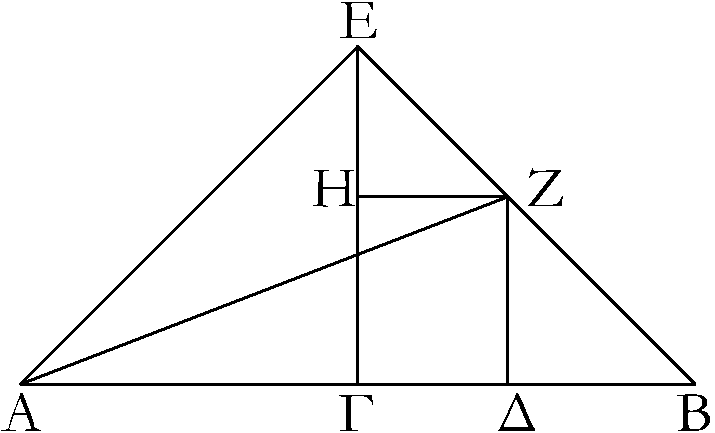
\includegraphics{Book02/fig09g.eps}}
 
\gr{Ἐὰν >άρα εὐθεῖα γραμμ\kern -.7pt  ὴ τμ\kern -.7pt  ηθῆ| εἰξ >ίσα καὶ >άνισα, τὰ ἀπὸ τῶν ἀνίσων τῆξ <όληξ τμ\kern -.5pt  ημάτων τετράγωνα διπλάσιά ἐστι τοῦ τε ἀπὸ τῆξ ἡμισείαξ καὶ τοῦ ἀπὸ τῆξ μεταχὺ τῶν τομῶν τετραγώνου;
<όπερ >έδει δεῖχαι.}}

\ParallelRText{
\begin{center}
{\large Proposition 9$^\dag$}
\end{center}

If a straight-line is cut into equal and unequal (pieces, then) the (sum of
the) squares on the unequal pieces of the whole (straight-line) is double
the (sum of the) square on half (the straight-line) and (the square) on the (difference)
between the (equal and unequal) pieces.

For let any straight-line $AB$ be cut---equally at $C$, and unequally
at $D$. I say that the (sum of the) squares on $AD$ and $DB$ is double
the (sum of the squares) on $AC$ and $CD$.

For let $CE$ be drawn from (point) $C$, at right-angles to $AB$ [Prop.~1.11], and let it be made equal to each of $AC$ and $CB$ [Prop.~1.3],
and let $EA$ and $EB$ be joined. And let $DF$ be drawn through
(point) $D$, parallel to $EC$ [Prop.~1.31], and (let) $FG$ (be drawn)
through (point) $F$, (parallel) to $AB$ [Prop.~1.31]. And let $AF$ be joined.
And since $AC$ is equal to $CE$,  the angle $EAC$ is also equal to the (angle) $AEC$ [Prop.~1.5]. And since the (angle) at $C$ is a right-angle, the (sum of the) remaining angles
(of triangle $AEC$), $EAC$ and $AEC$, is thus equal to one right-angle [Prop.~1.32].
And they are equal. Thus, (angles) $CEA$ and $CAE$ are each half a right-angle.
So, for the same (reasons), (angles) $CEB$ and $EBC$ are also each half a
right-angle. Thus, the whole (angle) $AEB$ is a right-angle. And since
$GEF$ is half a right-angle, and $EGF$ (is) a right-angle---for it is
equal to the internal and opposite  (angle) $ECB$ [Prop.~1.29]---the remaining (angle) $EFG$ is thus
half a right-angle [Prop.~1.32]. Thus, angle $GEF$ [is] equal to $EFG$.
So the side $EG$ is also equal to the (side) $GF$ [Prop.~1.6]. Again, since the angle
at $B$ is half a right-angle, and (angle) $FDB$ (is) a right-angle---for again
it is equal to the internal and opposite  (angle) $ECB$ [Prop.~1.29]---the
remaining (angle) $BFD$ is half a right-angle [Prop.~1.32]. Thus, the angle
at $B$ (is) equal to $DFB$. So the side $FD$ is also equal to the side $DB$ [Prop.~1.6]. And since $AC$ is equal to $CE$,  the (square) on $AC$ (is) also equal to the (square) on $CE$. Thus, the (sum of the) squares on $AC$ and $CE$
is double the (square) on $AC$. And the square on $EA$ is equal to the (sum
of the) squares on $AC$ and $CE$. For angle $ACE$ (is) 
a right-angle [Prop.~1.47].
Thus, the (square) on $EA$ is double the (square) on $AC$. Again,  since
$EG$ is equal to $GF$, the (square) on $EG$ (is) also equal  to 
the (square) on $GF$. 
Thus, the (sum of the squares)
on $EG$ and $GF$ is double the square on $GF$.
And the square on $EF$ is equal to the (sum of the) squares on $EG$ and $GF$
[Prop.~1.47]. Thus, the square on $EF$ is double the (square) on $GF$.
And $GF$ (is) equal to $CD$ [Prop.~1.34]. Thus, the (square) on $EF$ is double the
(square) on $CD$. And the (square) on $EA$ is also double the (square) on $AC$.
Thus, the (sum of the) squares on $AE$ and $EF$ is double the (sum of the)
squares on $AC$ and $CD$. And the square on $AF$ is equal to the
(sum of the squares) on $AE$ and $EF$. For the angle $AEF$ is a right-angle [Prop.~1.47]. Thus, the square on $AF$ is double the (sum of the squares) on 
$AC$ and $CD$. And the (sum of the squares) on $AD$ and $DF$ (is) equal to
the (square) on $AF$. For the angle at $D$ is a right-angle [Prop.~1.47].
Thus, the (sum of the squares) on $AD$ and $DF$ is double the (sum of the)
squares on $AC$ and $CD$. And $DF$ (is) equal to $DB$. Thus, the
(sum of the) squares on $AD$ and $DB$ is double the (sum of the) squares on
$AC$ and $CD$.

\epsfysize=1.8in
\centerline{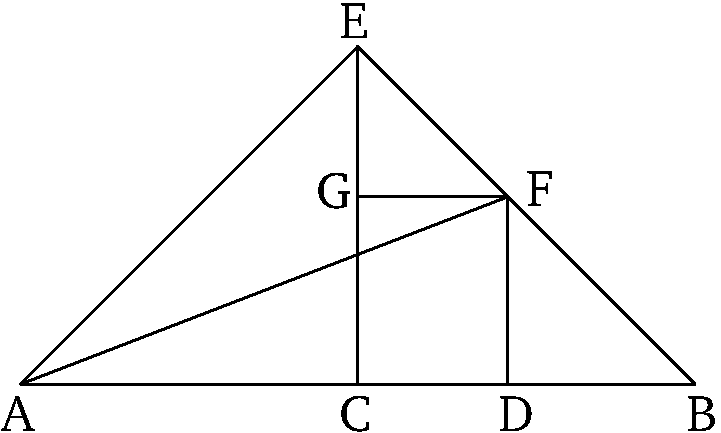
\includegraphics{Book02/fig09e.eps}}

Thus, if a straight-line is cut into equal and unequal (pieces, then) the (sum of the) squares on the unequal pieces of the whole (straight-line) is double
the (sum of the) square on half (the straight-line) and (the square) on the (difference)
between the (equal and unequal) pieces. (Which is) the very thing it was required to show.}
\end{Parallel}
{\footnotesize \noindent$^\dag$ This proposition is a geometric version
of the algebraic identity: $a^{\,2}+b^{\,2} = 2\left[\left([a+b]/2\right)^{\,2} + \left([a+b]/2-b\right)^{\,2}\right]$.}

%%%%%%
% Prop 2.10
%%%%%%
\pdfbookmark[1]{Proposition 2.10}{pdf2.10}
\begin{Parallel}{}{} 
\ParallelLText{
\begin{center}
{\large \ggn{10}.}
\end{center}\vspace*{-7pt}

\gr{Ἐὰν εὐθεῖα γραμμ\kern -.7pt  ὴ τμ\kern -.7pt  ηθῆ| δίθα, προστεθῆ| δέ τιξ α\kern -.5pt  ὐτῆ| εὐθεῖα  ἐπ> εὐθείαξ, τὸ ἀπὸ τῆξ <όληξ σὺν τῆ| προσκειμένῃ
καὶ τὸ ἀπὸ τῆξ προσκειμένηξ τὰ συναμφότερα τετράγωνα διπλάσιά ἐστι τοῦ τε ἀπὸ τῆξ ἡμισείαξ καὶ τοῦ ἀπὸ τῆξ συγκειμένηξ >έκ τε τῆξ ἡμισείαξ καὶ τῆξ προσκειμένηξ ὡξ ἀπὸ μιᾶξ ἀναγραφέντοξ τετραγώνου.}\\~\\

\epsfysize=2in
\centerline{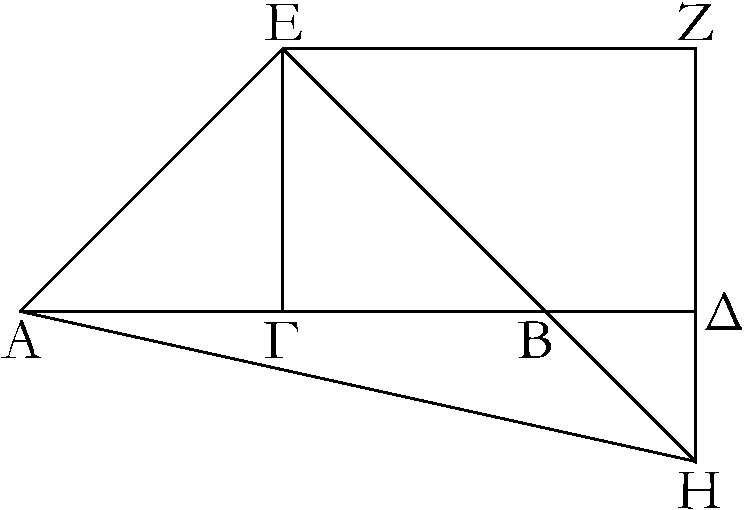
\includegraphics{Book02/fig10g.eps}}

\gr{Εὐθεῖα γάρ τιξ ἡ ΑΒ τετμ\kern -.7pt  ήσθω δίθα κατὰ τὸ Γ, προσκείσθω δέ τιξ α\kern -.7pt  ὐτῆ|
εὐθεῖα ἐπ> εὐθείαξ ἡ ΒΔ; λέγω, <ότι τὰ ἀπὸ τῶν ΑΔ, ΔΒ τετράγωνα διπλάσιά ἐστι τῶν ἀπὸ τῶν ΑΓ, ΓΔ τετραγώνων.}

\gr{>'Ηθθω γὰρ ἀπὸ τοῦ Γ σημείου τῆ| ΑΒ πρὸξ ὀρθὰξ ἡ ΓΕ, καὶ κείσθω >ίση ἑκατέρᾳ τῶν ΑΓ, ΓΒ, καὶ ἐπεζεύθθωσαν αἱ ΕΑ, ΕΒ; καὶ διὰ μὲν τοῦ Ε τῆ| ΑΔ παράλληλοξ >ήθθω ἡ ΕΖ, διὰ δὲ τοῦ Δ τῆ| ΓΕ παράλληλοξ >ήθθω ἡ ΖΔ. καὶ ἐπεὶ εἰξ παραλλήλουξ εὐθείαξ τὰξ ΕΓ, ΖΔ εὐθεῖά τιξ ἐνέπεσεν ἡ ΕΖ, αἱ ὑπὸ ΓΕΖ, ΕΖΔ >άρα δυσὶν ὀρθαῖξ >ίσαι εἰσίν; αἱ >άρα ὑπὸ ΖΕΒ, ΕΖΔ δύο ὀρθῶν ἐλάσσονέξ εἰσιν;
αἱ  δὲ ἀπ> ἐλασσόνων >ὴ δύο ὀρθῶν ἐκβαλλόμεναι συμπίπτουσιν;
αἱ >άρα ΕΒ, ΖΔ ἐκβαλλόμεναι ἐπὶ τὰ Β, Δ μέρη συμπεσοῦνται.
ἐκβεβλήσθωσαν καὶ συμπιπτέτωσαν κατὰ τὸ Η, καὶ ἐπεζεύθθω ἡ ΑΗ. καὶ ἐπεὶ >ίση ἐστὶν ἡ ΑΓ τῆ| ΓΕ, >ίση ἐστὶ καὶ γωνία ἡ ὑπὸ ΕΑΓ τῆ| ὑπὸ ΑΕΓ; καὶ ὀρθὴ ἡ πρὸξ τῶ| Γ; ἡμίσεια >άρα 
ὀρθῆξ [ἐστιν] ἑκατέρα τῶν ὑπὸ ΕΑΓ, ΑΕΓ. διὰ τὰ α\kern -.7pt  ὐτὰ δὴ καὶ ἑκατέρα τῶν ὑπὸ ΓΕΒ, ΕΒΓ ἡμίσειά ἐστιν ὀρθῆξ; ὀρθὴ >άρα ἐστὶν ἡ ὑπὸ ΑΕΒ. καὶ ἐπεὶ ἡμίσεια ὀρθῆξ ἐστιν ἡ ὑπὸ ΕΒΓ, ἡμίσεια >άρα 
ὀρθῆξ καὶ ἡ ὑπὸ ΔΒΗ. >έστι δὲ καὶ ἡ 
ὑπὸ ΒΔΗ ὀρθή; >ίση γάρ ἐστι τῆ| ὑπὸ ΔΓΕ; ἐναλλὰχ γάρ; 
λοιπὴ <άρα ἡ ὑπὸ ΔΗΒ ἡμίσειά ἐστιν ὀρθῆξ; ἡ 
>άρα ὑπὸ ΔΗΒ τῆ| ὑπὸ ΔΒΗ ἐστιν >ίση; <ώστε καὶ πλευρὰ ἡ ΒΔ πλευρᾶ| τῆ| ΗΔ ἐστιν >ίση.
πάλιν, ἐπεὶ ἡ ὑπὸ ΕΗΖ ἡμίσειά ἐστιν ὀρθῆξ, ὀρθὴ δὲ ἡ πρὸξ τῶ| Ζ; >ίση γάρ ἐστι τῆ| ἀπεναντίον τῆ| πρὸξ τῶ| Γ; λοιπὴ >άρα ἡ ὑπὸ ΖΕΗ ἡμίσειά ἐστιν
ὀρθῆξ;  >ίση >άρα ἡ ὑπὸ ΕΗΖ γωνία τῆ| ὑπὸ ΖΕΗ; <ώστε
καὶ πλευρὰ ἡ ΗΖ πλευρᾶ| τῆ| ΕΖ ἐστιν >ίση. καὶ ἐπεὶ [>ίση ἐστὶν ἡ ΕΓ τῆ| ΓΑ], >ίσον ἐστὶ [καὶ] τὸ ἀπὸ τῆξ ΕΓ τετράγωνον τῶ| ἀπὸ τῆξ ΓΑ τετραγώνῳ; τὰ >άρα ἀπὸ τῶν ΕΓ, ΓΑ τετράγωνα διπλάσιά
ἐστι τοῦ ἀπὸ τῆξ ΓΑ τετραγώνου. τοῖξ δὲ ἀπὸ τῶν ΕΓ, ΓΑ >ίσον
ἐστὶ τὸ ἀπὸ τῆξ ΕΑ; τὸ >άρα ἀπὸ τῆξ ΕΑ τετράγωνον διπλάσιόν ἐστι τοῦ ἀπὸ τῆξ ΑΓ τετραγώνου. πάλιν, ἐπεὶ >ίση ἐστὶν ἡ ΖΗ τῆ| ΕΖ, 
>ίσον ἐστὶ καὶ τὸ ἀπὸ τῆξ ΖΗ τῶ| ἀπὸ τῆξ ΖΕ; τὰ >άρα ἀπὸ τῶν ΗΖ, ΖΕ διπλάσιά ἐστι τοῦ ἀπὸ τῆξ ΕΖ. τοῖξ δὲ ἀπὸ τῶν ΗΖ, ΖΕ
>ίσον ἐστὶ τὸ ἀπὸ τῆξ ΕΗ; τὸ >άρα ἀπὸ τῆξ ΕΗ διπλάσιόν ἐστι
τοῦ ἀπὸ τῆξ ΕΖ. >ίση δὲ ἡ ΕΖ τῆ| ΓΔ; τὸ >άρα ἀπὸ τῆξ ΕΗ τετράγωνον διπλάσιόν ἐστι τοῦ ἀπὸ τῆξ ΓΔ. ἐδείθθη δὲ καὶ τὸ ἀπὸ τῆξ ΕΑ διπλάσιον
τοῦ ἀπὸ τῆξ ΑΓ; τὰ >άρα ἀπὸ τῶν ΑΕ, ΕΗ τετράγωνα διπλάσιά ἐστι τῶν ἀπὸ τῶν ΑΓ, ΓΔ τετραγώνων. τοῖξ
δὲ ἀπὸ τῶν ΑΕ, ΕΗ τετραγώνοιξ >ίσον ἐστὶ τὸ ἀπὸ τῆξ ΑΗ τετράγωνον; τὸ >άρα ἀπὸ τῆξ ΑΗ διπλάσιόν ἐστι τῶν ἀπὸ τῶν ΑΓ, ΓΔ. τῶ| δὲ ἀπὸ τῆξ ΑΗ >ίσα ἐστὶ τὰ ἀπὸ τῶν ΑΔ, ΔΗ; τὰ >άρα
ἀπὸ τῶν ΑΔ, ΔΗ [τετράγωνα] διπλάσιά ἐστι τῶν ἀπὸ τῶν ΑΓ, ΓΔ [τετραγώνων]. >ίση δὲ ἡ ΔΗ τῆ| ΔΒ; τὰ >άρα ἀπὸ τῶν ΑΔ, ΔΒ [τετράγωνα] διπλάσιά ἐστι τῶν ἀπὸ τῶν ΑΓ, ΓΔ τετραγώνων.}

\gr{Ἐὰν >άρα εὐθεῖα γραμμ\kern -.7pt  ὴ τμ\kern -.7pt  ηθῆ| δίθα, προστεθῆ| δέ τιξ α\kern -.5pt  ὐτῆ| εὐθεῖα  ἐπ> εὐθείαξ, τὸ ἀπὸ τῆξ <όληξ σὺν τῆ| προσκειμένῃ
καὶ τὸ ἀπὸ τῆξ προσκειμένηξ τὰ συναμφότερα τετράγωνα διπλάσιά ἐστι τοῦ τε ἀπὸ τῆξ ἡμισείαξ καὶ τοῦ ἀπὸ τῆξ συγκειμένηξ >έκ τε τῆξ ἡμισείαξ καὶ τῆξ προσκειμένηξ ὡξ ἀπὸ μιᾶξ ἀναγραφέντοξ τετραγώνου; <όπερ >έδει δεῖχαι.}}

\ParallelRText{
\begin{center}
{\large Proposition 10$^\dag$}
\end{center}

If a straight-line is cut in half, and any straight-line added to it straight-on,
(then) the sum of the square on the whole (straight-line) with the (straight-line) having
been added, and the (square) on the (straight-line) having been added, 
is double the (sum of the square) on half (the straight-line), and
the square described on the sum of half (the straight-line) and (straight-line)
having been added, as on one (complete straight-line).

\epsfysize=2in
\centerline{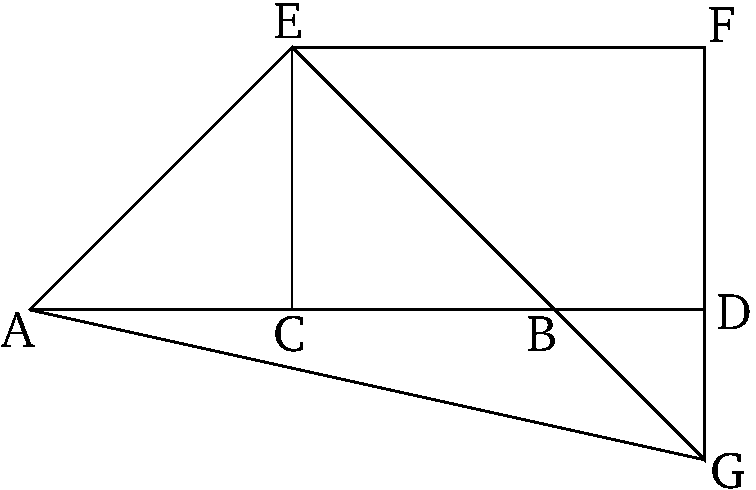
\includegraphics{Book02/fig10e.eps}}

For let any straight-line $AB$ be cut in half at (point) $C$, and let any
straight-line $BD$ be added to it straight-on. I say that the
(sum of the) squares on $AD$ and $DB$ is double the (sum of the) squares on $AC$ and $CD$.

For let $CE$ be drawn from point $C$, at right-angles to $AB$ [Prop.~1.11],
and let it be made equal to each of $AC$ and $CB$ [Prop.~1.3], and let $EA$ and
$EB$ be joined. And let $EF$ be drawn through $E$, parallel to $AD$
[Prop.~1.31], and let $FD$ be drawn through $D$, parallel to $CE$ [Prop.~1.31]. And since some straight-line $EF$ falls across the parallel straight-lines $EC$ and $FD$, the (internal angles) $CEF$ and $EFD$ are thus equal
to two right-angles [Prop.~1.29]. Thus, $FEB$ and $EFD$ are less than two
right-angles. And (straight-lines) produced from (internal angles whose sum is) less than
two right-angles meet together [Post.~5]. Thus, being produced in the direction of $B$
and $D$, the (straight-lines) $EB$ and $FD$ will meet. Let them be 
produced,
and let them meet together at $G$, and let $AG$ be joined.
And since $AC$ is equal to $CE$, angle $EAC$ is also equal to (angle) $AEC$ [Prop.~1.5]. And the (angle) at $C$ (is) a right-angle. Thus, $EAC$ and $AEC$
[are] each half a right-angle [Prop.~1.32]. So, for the same (reasons), $CEB$ and $EBC$ are
also each half a right-angle. Thus, (angle) $AEB$ is a right-angle.
And since $EBC$ is half a right-angle, $DBG$ (is) thus also half a right-angle
[Prop.~1.15]. And $BDG$ is also a right-angle. For it is equal to $DCE$.
For (they are) alternate (angles) [Prop.~1.29].
Thus, the remaining (angle) $DGB$ is half a right-angle. Thus,
$DGB$ is equal to $DBG$. So side $BD$ is also equal to side $GD$ [Prop.~1.6].
Again, 
since $EGF$ is  half a right-angle, and the (angle) at $F$ (is) a right-angle,
for it is equal to the opposite (angle) at $C$
[Prop.~1.34], the remaining
(angle) $FEG$ is thus half a right-angle. Thus, angle $EGF$ (is) equal to $FEG$.
So the side $GF$ is also equal to the side $EF$ [Prop.~1.6].
And since [$EC$ is equal to $CA$] the square on $EC$ is [also] equal to the
square on $CA$. Thus, the (sum of the) squares on $EC$ and $CA$ is 
double the square on $CA$. And the (square) on $EA$ is equal to the (sum of the
squares) on $EC$ and $CA$ [Prop.~1.47]. Thus, the square on $EA$ is double the
square on $AC$. Again, since $FG$ is equal to $EF$, the (square) on $FG$ is also
equal to the (square) on $FE$. Thus, the (sum of the squares) on $GF$ and
$FE$ is double the (square) on $EF$. And the (square) on $EG$ is equal to
the (sum of the squares) on  $GF$ and $FE$ [Prop.~1.47]. Thus, the (square)
on $EG$ is double the (square) on $EF$. And $EF$ (is) equal to $CD$  [Prop.~1.34].
Thus, the square on $EG$ is double the (square) on $CD$. But it was also
shown that the (square) on $EA$ (is) double the (square) on $AC$. Thus,
the (sum of the) squares on $AE$ and $EG$ is double the (sum of the) squares
on $AC$ and $CD$. And the square on $AG$ is equal to the (sum of the) squares
on $AE$ and $EG$ [Prop.~1.47]. Thus, the (square) on $AG$ is double the (sum of the squares) on $AC$ and $CD$. And the (sum of the squares) on $AD$ and $DG$ 
is equal to the (square) on $AG$  [Prop.~1.47].
Thus, the (sum of the) [squares] on $AD$ and $DG$ is double the
(sum of the) [squares] on $AC$ and $CD$. And $DG$ (is) equal to $DB$.
Thus, the (sum of the) [squares] on $AD$ and $DB$ is double the
(sum of the) squares on $AC$ and $CD$. 

Thus, if a straight-line is cut in half, and any straight-line added to it straight-on,
(then) the sum of the square on the whole (straight-line) with the (straight-line) having
been added, and the (square) on the (straight-line) having been added, 
is double the (sum of the square) on half (the straight-line), and
the square described on the sum of half (the straight-line) and (straight-line)
having been added, as on one (complete straight-line). (Which is) the
very thing it was required to show.}
\end{Parallel}
{\footnotesize \noindent$^\dag$ This proposition is a geometric version
of the algebraic identity: $(2\,a+b)^{\,2}+b^{\,2}= 2\,\left[a^{\,2}+(a+b)^{\,2}\right]$.}

%%%%%%
% Prop 2.11
%%%%%%
\pdfbookmark[1]{Proposition 2.11}{pdf2.11}
\begin{Parallel}{}{} 
\ParallelLText{
\begin{center}
{\large \ggn{11}.}
\end{center}\vspace*{-7pt}

\gr{Τὴν δοθεῖσαν εὐθεῖαν τεμεῖν <ώστε τὸ ὑπὸ τῆξ <όληξ καὶ
τοῦ ἑτέρου τῶν τμ\kern -.7pt  ημάτων περιεχόμενον ὀρθογώνιον >ίσον ε>ῖναι
τῶ| ἀπὸ τοῦ λοιποῦ τμ\kern -.7pt  ήματοξ τετραγώνῳ.}

\gr{>'Εστω ἡ δοθεῖσα εὐθεῖα ἡ ΑΒ; δεῖ δὴ τὴν ΑΒ τεμεῖν <ώστε
τὸ ὑπὸ τῆξ <όληξ καὶ τοῦ ἑτέρου τῶν τμ\kern -.7pt  ημάτων περιεχόμενον ὀρθογώνιον >ίσον ε>ῖναι τῶ| ἀπὸ τοῦ λοιποῦ τμ\kern -.7pt  ήματοξ τετραγώνῳ.}\\

\epsfysize=2.75in
\centerline{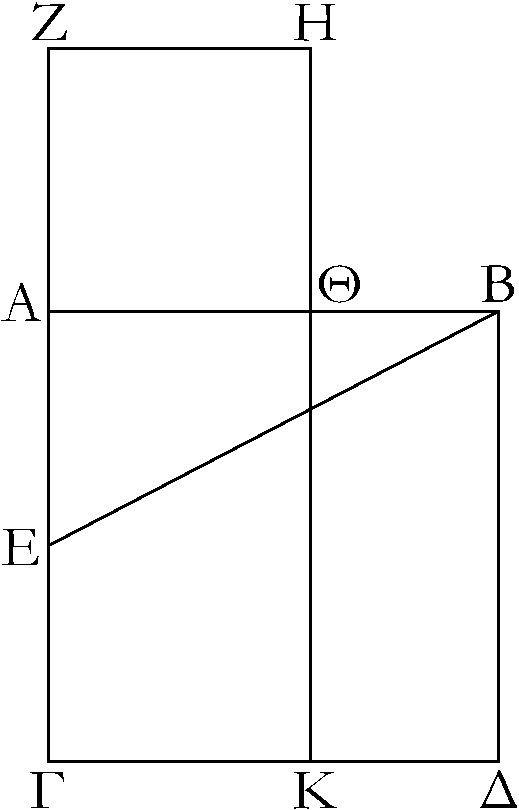
\includegraphics{Book02/fig11g.eps}}

\gr{Ἀναγεγράφθω γὰρ ἀπὸ τῆξ ΑΒ τετράγωνον τὸ ΑΒΔΓ, καὶ τετμ\kern -.7pt  ήσθω ἡ ΑΓ δίθα κατὰ τὸ Ε σημεῖον, καὶ ἐπεζεύθθω ἡ ΒΕ, καὶ διήθθω ἡ ΓΑ ἐπὶ τὸ Ζ, καὶ κείσθω τῆ| ΒΕ >ίση ἡ ΕΖ, καὶ ἀναγεγράφθω ἀπὸ
τῆξ ΑΖ τετράγωνον τὸ ΖJ, καὶ
διήθθω ἡ ΗJ ἐπὶ τὸ Κ; λέγω, <ότι ἡ ΑΒ τέτμ\kern -.7pt  ηται κατὰ τὸ J, <ώστε τὸ ὑπὸ τῶν ΑΒ, ΒJ περιεχόμενον ὀρθογώνιον >ίσον ποιεῖν τῶ| ἀπὸ τῆξ ΑJ τετραγώνῳ.}

\gr{Ἐπεὶ γὰρ εὐθεῖα ἡ ΑΓ τέτμ\kern -.7pt  ηται δίθα κατὰ τὸ Ε, πρόσκειται δὲ α\kern -.7pt  ὐτῆ| ἡ ΖΑ, τὸ >άρα ὑπὸ τῶν ΓΖ, ΖΑ περιεχόμενον ὀρθογώνιον μετὰ τοῦ ἀπὸ τῆξ ΑΕ τετραγώνου >ίσον ἐστὶ τῶ| ἀπὸ τῆξ ΕΖ τετραγώνῳ. >ίση δὲ ἡ ΕΖ τῆ| ΕΒ; τὸ >άρα ὑπὸ τῶν ΓΖ, ΖΑ μετὰ τοῦ ἀπὸ τῆξ ΑΕ >ίσον ἐστὶ τῶ| ἀπὸ ΕΒ. ἀλλὰ τῶ| ἀπὸ 
ΕΒ >ίσα ἐστὶ τὰ ἀπὸ τῶν ΒΑ, ΑΕ; ὀρθὴ γὰρ ἡ πρὸξ τῶ| Α γωνία; τὸ >άρα ὑπὸ τῶν ΓΖ, ΖΑ μετὰ τοῦ ἀπὸ τῆξ ΑΕ >ίσον ἐστὶ τοῖξ ἀπὸ τῶν ΒΑ, ΑΕ. κοινὸν ἀφῃρήσθω τὸ ἀπὸ τῆξ ΑΕ; λοιπὸν >άρα τὸ ὑπὸ τῶν ΓΖ, ΖΑ
περιεχόμενον ὀρθογώνιον >ίσον ἐστὶ τῶ| ἀπὸ τῆξ ΑΒ τετραγώνῳ.
καί ἐστι τὸ μὲν ὑπὸ τῶν ΓΖ, ΖΑ τὸ ΖΚ; >ίση γὰρ ἡ ΑΖ τῆ| ΖΗ;
τὸ δὲ ἀπὸ τῆξ ΑΒ τὸ ΑΔ; τὸ >άρα ΖΚ >ίσον ἐστὶ τῶ| ΑΔ. κοινὸν ἀρῃρήσθω τὸ ΑΚ; λοιπὸν >άρα τὸ ΖJ τῶ| JΔ >ίσον ἐστίν. καί ἐστι τὸ μὲν JΔ τὸ ὑπὸ τῶν ΑΒ, ΒJ; 
>ίση γὰρ ἡ ΑΒ τῆ| ΒΔ; τὸ δὲ ΖJ τὸ ἀπὸ τῆξ ΑJ; τὸ >άρα ὑπὸ τῶν ΑΒ, ΒJ περιεχόμενον ὀρθογώνιον >ίσον ἐστὶ τῶ| ἀπὸ JΑ τετραγώνῳ.}

\gr{Ἡ  >άρα δοθεῖσα εὐθεῖα ἡ ΑΒ τέτμ\kern -.7pt  ηται 
κατὰ τὸ J <ώστε τὸ ὑπὸ τῶν ΑΒ, ΒJ 
περιεχόμενον ὀρθογώνιον >ίσον ποιεῖν
τῶ| ἀπὸ τῆξ JΑ τετραγώνῳ; <όπερ >έδει ποιῆσαι.}}

\ParallelRText{
\begin{center}
{\large Proposition 11$^\dag$}
\end{center}

To cut a given straight-line such that the rectangle contained by the whole (straight-line), and one of the pieces (of the straight-line), is equal to the
square on the remaining piece.

Let $AB$ be the given straight-line. So it is required to cut $AB$ such that the rectangle contained by the whole (straight-line), and one of the
pieces (of the straight-line), is equal to the square on the remaining piece.

\epsfysize=2.75in
\centerline{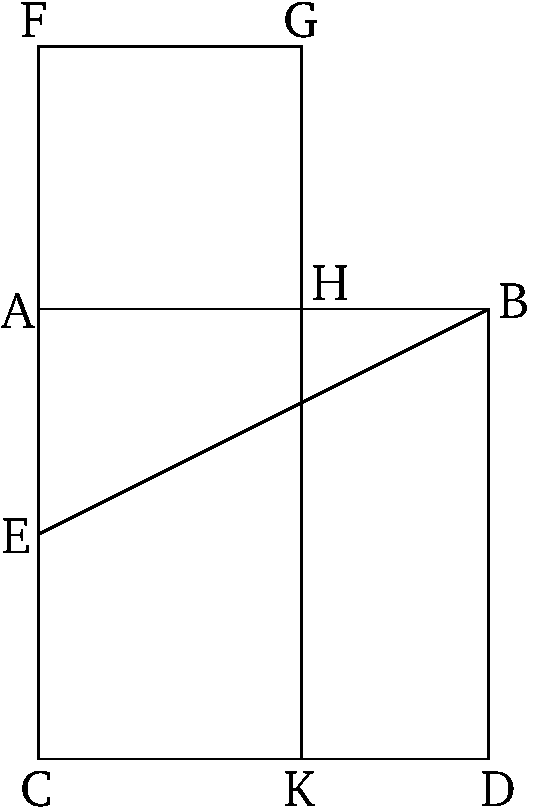
\includegraphics{Book02/fig11e.eps}}

For let the square $ABDC$ be described on $AB$ [Prop.~1.46],
and let $AC$ be cut in half at point $E$ [Prop.~1.10], and
let $BE$ be joined.  And let $CA$ be drawn through to (point)
$F$, and let $EF$ be made equal to $BE$ [Prop.~1.3]. And let the square $FH$ 
be described on $AF$ [Prop.~1.46], and let $GH$ be drawn
through to (point) $K$. I say that $AB$ has been cut at $H$ such as to make the
rectangle contained by $AB$ and $BH$ equal to the square on $AH$.

For since the straight-line $AC$ has been cut in half at $E$, and $FA$ has been
added to it, the rectangle contained by $CF$ and $FA$, plus the square on $AE$, is
thus equal to the square on $EF$ [Prop.~2.6]. And $EF$ (is) equal to $EB$. Thus,
the (rectangle contained) by $CF$ and $FA$, plus the (square) on $AE$, is equal
to the (square) on $EB$. But, the (sum of the squares) on $BA$ and $AE$ is equal
to the (square) on $EB$. For the angle at $A$ (is) a right-angle [Prop.~1.47].
Thus, the (rectangle contained) by $CF$ and $FA$, plus the (square) on $AE$,
is equal to the (sum of the squares) on $BA$ and $AE$. Let the square on $AE$ have
been subtracted from both. Thus, the remaining rectangle contained by
$CF$ and $FA$ is equal to the square on $AB$.  And $FK$ is the (rectangle contained)
by $CF$ and $FA$. For $AF$ (is) equal to $FG$. And $AD$ (is) the (square) on $AB$. Thus, the
(rectangle) $FK$ is equal to the (square) $AD$. Let (rectangle) $AK$ be
subtracted from both. Thus, the remaining (square) $FH$ is equal to 
the (rectangle) $HD$. And  $HD$ is the (rectangle contained) by $AB$ and $BH$.
For $AB$ (is) equal to $BD$. And $FH$ (is) the (square) on $AH$.
Thus, the rectangle contained by $AB$ and $BH$ is equal to the square on $HA$.

Thus, the given straight-line $AB$ has been cut at (point) $H$ such as to make
the rectangle contained by $AB$ and $BH$ equal to the square on $HA$.
(Which is) the very thing it was required to do.
}
\end{Parallel}
{\footnotesize \noindent$^\dag$ This manner of cutting a straight-line---so
that the ratio of the whole to the larger piece is equal to the ratio
of the larger to the smaller piece---is sometimes called the ``Golden Section''.}

%%%%%%
% Prop 2.12
%%%%%%
\pdfbookmark[1]{Proposition 2.12}{pdf2.12}
\begin{Parallel}{}{} 
\ParallelLText{
\begin{center}

{\large\ggn{12}.}
\end{center}\vspace*{-7pt}

\gr{Ἐν τοῖξ ἀμβλυγωνίοιξ τριγώνοιξ τὸ ἀπὸ τῆξ τὴν ἀμβλεῖαν
γωνίαν ὑποτεινούσηξ πλευρᾶξ τετράγωνον μεῖζόν ἐστι τῶν ἀπὸ
τῶν τὴν ἀμβλεῖαν γωνίαν περιεθουσῶν πλευρῶν τετραγώνων τῶ| περιεθομένῳ δὶξ
ὑπὸ τε μιᾶξ τῶν περὶ τὴν ἀμβλεῖαν γωνίαν, ἐφ> <ὴν ἡ
κάθετοξ πίπτει, καὶ τῆξ ἀπολαμβανομένηξ ἐκτὸξ ὑπὸ τῆξ
καθέτου πρὸξ τῆ| ἀμβλείᾳ γωνίᾳ.}

\gr{>'Εστω ἀμβλυγώνιον τρίγωνον τὸ ΑΒΓ ἀμβλεῖαν >έθον τὴν ὑπὸ
ΒΑΓ, καὶ >ήθθω ἀπὸ τοῦ Β σημείου ἐπὶ τὴν ΓΑ ἐκβληθεῖσαν κάθετοξ ἡ ΒΔ. λέγω, <ότι τὸ ἀπὸ τῆξ ΒΓ τετράγωνον μεῖζόν ἐστι
τῶν ἀπὸ τῶν ΒΑ, ΑΓ τετραγώνων τῶ| δὶξ ὑπὸ τῶν ΓΑ, ΑΔ περιεθομένῳ ὀρθογωνίῳ.}\\

\epsfysize=1.8in
\centerline{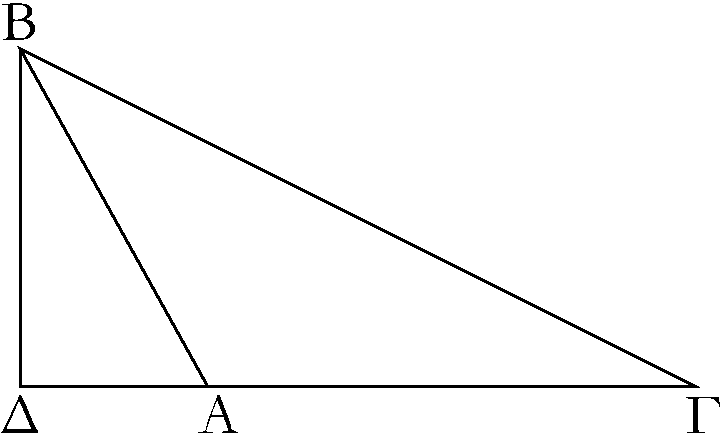
\includegraphics{Book02/fig12g.eps}}

\gr{Ἐπεὶ γὰρ εὐθεῖα ἡ ΓΔ τέτμ\kern -.7pt  ηται, ὡξ >έτυθεν, κατὰ τὸ Α σημεῖον,
τὸ >άρα ἀπὸ τῆξ ΔΓ >ίσον ἐστὶ τοῖξ ἀπὸ τῶν ΓΑ, ΑΔ τετραγώνοιξ καὶ τῶ| δὶξ ὑπὸ τῶν ΓΑ, ΑΔ περιεθομένῳ ὀρθογωνίῳ. κοινὸν προσκείσθω τὸ ἀπὸ τῆξ ΔΒ; τὰ >άρα ἀπὸ τῶν ΓΔ, ΔΒ >ίσα ἐστὶ
τοῖξ τε ἀπὸ τῶν ΓΑ, ΑΔ, ΔΒ τετραγώνοιξ καὶ τῶ| δὶξ ὑπὸ
τῶν ΓΑ, ΑΔ [περιεθομένῳ ὀρθογωνίῳ]. ἀλλὰ τοῖξ μὲν ἀπὸ τῶν
ΓΔ, ΔΒ >ίσον ἐστὶ τὸ ἀπὸ τῆξ ΓΒ;
ὀρθὴ γὰρ ἡ προξ τῶ| Δ γωνία; τοῖξ δὲ ἀπὸ τῶν ΑΔ, ΔΒ >ίσον τὸ ἀπὸ τῆξ ΑΒ; τὸ >άρα ἀπὸ τῆξ ΓΒ τετράγωνον >ίσον ἐστὶ τοῖξ τε
ἀπὸ τῶν ΓΑ, ΑΒ
τετραγώνοιξ καὶ τῶ| δὶξ ὑπὸ
τῶν ΓΑ, ΑΔ περιεθομένῳ ὀρθογωνίῳ; <ώστε τὸ ἀπὸ τῆξ ΓΒ
τετράγωνον τῶν ἀπὸ τῶν ΓΑ, ΑΒ τετραγώνων μεῖζόν
ἐστι τῶ| δὶξ ὑπὸ τῶν ΓΑ, ΑΔ περιεθομένῳ ὀρθογωνίῳ.}

\gr{Ἐν >άρα τοῖξ ἀμβλυγωνίοιξ τριγώνοιξ τὸ ἀπὸ τῆξ τὴν ἀμβλεῖαν
γωνίαν ὑποτεινούσηξ πλευρᾶξ τετράγωνον μεῖζόν ἐστι τῶν ἀπὸ
τῶν τὴν ἀμβλεῖαν γωνίαν περιεθουσῶν πλευρῶν τετραγώνων τῶ| περιθομένῳ δὶξ ὑπό τε μιᾶξ τῶν περὶ τὴν ἀμβλεῖαν γωνίαν, ἐφ> <ὴν ἡ
κάθετοξ πίπτει, καὶ τῆξ ἀπολαμβανομένηξ ἐκτὸξ ὑπὸ τῆξ
καθέτου πρὸξ τῆ| ἀμβλείᾳ γωνίᾳ; <όπερ >έδει δεῖχαι.}}

\ParallelRText{
\begin{center}
{\large Proposition 12$^\dag$}
\end{center}

In obtuse-angled triangles, the square on the side subtending the obtuse
angle is greater than the (sum of the) squares on the sides containing the obtuse angle
by twice the (rectangle) contained by one of the sides around the obtuse
angle, to which a perpendicular (straight-line) falls, and the 
 (straight-line) cut off outside (the triangle)
 by the perpendicular (straight-line) towards the obtuse angle.
 
 Let $ABC$ be an obtuse-angled triangle, having the 
 angle $BAC$ obtuse. And let $BD$ be drawn from point $B$, perpendicular
 to $CA$ produced [Prop.~1.12]. I say that the square on $BC$ is greater than the
 (sum of the) squares on $BA$ and $AC$ by twice the rectangle contained
 by $CA$ and $AD$.
  
\epsfysize=1.8in
\centerline{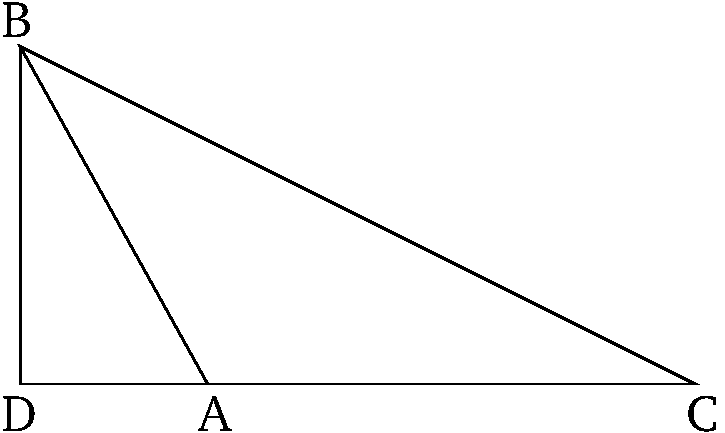
\includegraphics{Book02/fig12e.eps}}

 For since the straight-line $CD$ has been cut, at random, at point $A$, 
 the (square) on $DC$ is thus equal to the (sum of the) squares on $CA$ and $AD$,
 and twice the rectangle contained by $CA$ and $AD$ [Prop.~2.4]. Let
 the (square) on $DB$ be added to both. Thus, the
 (sum of the squares) on $CD$ and $DB$ is equal to the (sum of the) squares
 on $CA$, $AD$, and $DB$, and twice the [rectangle contained] by $CA$ and $AD$.
 But, the (square) on
 $CB$ is equal to the (sum of the squares) on $CD$ and $DB$. For the angle at $D$ (is) a right-angle [Prop.~1.47]. And  the (square) on 
 $AB$ (is) equal to the (sum of the
 squares) on $AD$ and $DB$  [Prop.~1.47]. Thus, the square on $CB$ is equal to the (sum of the)
 squares on $CA$ and $AB$, and twice the rectangle contained by $CA$ and $AD$.  So the square on $CB$ is greater than the (sum of the) squares on $CA$ and
 $AB$ by twice the rectangle contained by $CA$ and $AD$.
 
Thus, in  obtuse-angled triangles, the square on the side subtending the obtuse
angle is greater than the (sum of the) squares on the sides containing the obtuse angle
by twice the (rectangle) contained by one of the sides around the obtuse
angle, to which a perpendicular (straight-line) falls, and the 
 (straight-line) cut off outside (the triangle)
 by the perpendicular (straight-line) towards the obtuse angle.
 (Which is) the very thing it was required to show.}
\end{Parallel}
{\footnotesize \noindent$^\dag$ This proposition is equivalent
to the well-known cosine formula: $BC^{\,2} = AB^{\,2} + AC^{\,2} -2\,AB\,AC\,\cos BAC$, since $\cos BAC = - AD / AB$.}

%%%%%%
% Prop 2.13
%%%%%%
\pdfbookmark[1]{Proposition 2.13}{pdf2.13}
\begin{Parallel}{}{} 
\ParallelLText{
\begin{center}
{\large\ggn{13}.}
\end{center}\vspace*{-7pt}

\gr{Ἐν τοῖξ ὀχυγωνίοιξ τριγώνοιξ τὸ ἀπὸ τῆξ τὴν  ὀχεῖαν γωνίαν
ὑποτεινούσηξ πλευρᾶξ τετράγωνον >έλαττόν ἐστι τῶν ἀπὸ τῶν
τὴν ὀχεῖαν γωνίαν περιεθουσῶν πλευρῶν τετραγώνων τῶ|
περιεθομένῳ δὶξ ὑπό τε μιᾶξ τῶν περὶ τὴν ὀχεῖαν γωνίαν, ἐφ>
<ὴν ἡ κάθετοξ πίπτει, καὶ τῆξ ἀπολαμβανομένηξ ἐντὸξ ὑπὸ
τῆξ καθέτου πρὸξ τῆ| ὀχείᾳ γωνίᾳ.}\\

\epsfysize=2in
\centerline{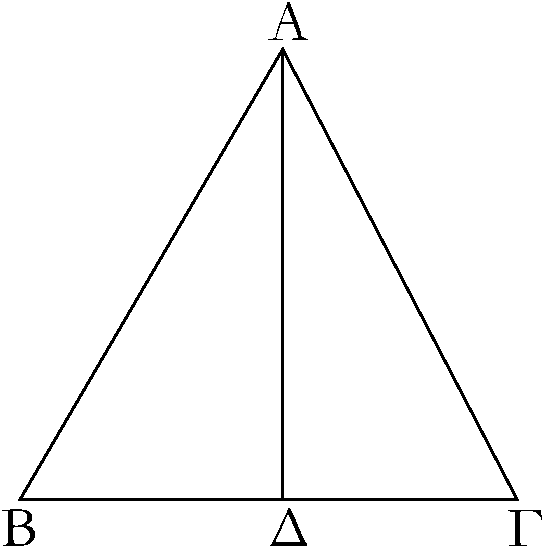
\includegraphics{Book02/fig13g.eps}}

\gr{>'Εστω ὀχυγώνιον τρίγωνον τὸ ΑΒΓ ὀχεῖαν >έθον τὴν πρὸξ τῶ|
Β γωνίαν, καὶ >ήθθω ἀπὸ τοῦ Α σημείου ἐπὶ τὴν ΒΓ κάθετοξ
ἡ ΑΔ; λέγω, <ότι τὸ ἀπὸ τῆξ ΑΓ τετράγωνον >έλαττόν ἐστι τῶν
ἀπὸ τῶν ΓΒ, ΒΑ τετραγώνων τῶ| δὶξ ὑπὸ τῶν ΓΒ, ΒΔ περιεθομένῳ ὀρθογωνίῳ.}

\gr{Ἐπεὶ γὰρ εὐθεῖα ἡ ΓΒ τέτμ\kern -.7pt  ηται, ὡξ >έτυθεν, κατὰ τὸ Δ, τὰ >άρα ἀπὸ τῶν ΓΒ, ΒΔ τετράγωνα >ίσα ἐστὶ τῶ| τε δὶξ ὑπὸ τῶν ΓΒ, ΒΔ
περιεθομένῳ ὀρθογωνίῳ καὶ τῶ| ἀπὸ τῆξ ΔΓ τετραγώνῳ. κοινὸν προσκείσθω τὸ ἀπὸ τῆξ ΔΑ τετράγωνον; τὰ >άρα ἀπὸ τῶν ΓΒ, ΒΔ, ΔΑ
τετράγωνα >ίσα ἐστὶ τῶ| τε δὶξ ὑπὸ τῶν ΓΒ, ΒΔ περιεθομένῳ
ὀρθογωνίῳ καὶ τοῖξ ἀπὸ τῶν ΑΔ, ΔΓ τετραγώνιοξ. ἀλλὰ τοῖξ
μὲν ἀπὸ τῶν ΒΔ, ΔΑ >ίσον τὸ ἀπὸ τῆξ ΑΒ; ὀρθὴ γὰρ ἡ πρὸξ
τῶ| Δ γωνίᾳ; τοῖξ δὲ ἀπὸ τῶν ΑΔ, ΔΓ >ίσον τὸ ἀπὸ τῆξ
ΑΓ; τὰ >άρα ἀπὸ τῶν
 ΓΒ, ΒΑ >ίσα ἐστὶ τῶ| τε ἀπὸ
τῆξ ΑΓ καὶ τῶ| δὶξ ὑπὸ τῶν ΓΒ, ΒΔ; <ώστε μόνον τὸ ἀπὸ τῆξ ΑΓ >έλαττόν ἐστι τῶν ἀπὸ τῶν ΓΒ, ΒΑ τετραγώνων τῶ| δὶξ
ὑπὸ τῶν ΓΒ, ΒΔ περιεθομένῳ ὀρθογωνίῳ.}

\gr{Ἐν >άρα τοῖξ ὀχυγωνίοιξ τριγώνοιξ τὸ ἀπὸ τῆξ τὴν  ὀχεῖαν γωνίαν
ὑποτεινούσηξ πλευρᾶξ τετράγωνον >έλαττόν ἐστι τῶν ἀπὸ τῶν
τὴν ὀχεῖαν γωνίαν περιεθουσῶν πλευρῶν τετραγώνων τῶ|
περιεθομένῳ δὶξ ὑπό τε μιᾶξ τῶν περὶ τὴν ὀχεῖαν γωνίαν, ἐφ>
<ὴν ἡ κάθετοξ πίπτει, καὶ τῆξ ἀπολαμβανομένηξ ἐντὸξ ὑπὸ
τῆξ καθέτου πρὸξ τῆ| ὀχείᾳ γωνίᾳ; <όπερ >έδει δεῖχαι.}}

\ParallelRText{
\begin{center}
{\large Proposition 13$^\dag$}
\end{center}

In acute-angled triangles, the square on the side subtending the acute angle
is less than the (sum of the) squares on the sides containing the acute
angle by twice the (rectangle) contained by one of the sides around the acute
angle, to which a perpendicular (straight-line) falls, and the 
 (straight-line) cut off inside (the triangle)
 by the perpendicular (straight-line) towards the acute angle.
 
 \epsfysize=2in
\centerline{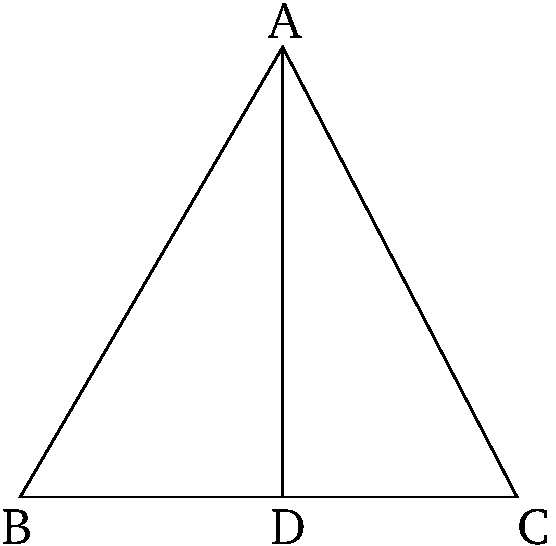
\includegraphics{Book02/fig13e.eps}}

 Let $ABC$ be an acute-angled triangle, having the  angle at (point) $B$ acute.
 And let $AD$ be drawn from point $A$, perpendicular to $BC$ [Prop.~1.12].
I say that the square on $AC$ is less than the (sum of the) squares on $CB$ and $BA$ by twice the rectangle contained by $CB$ and $BD$.

For since the straight-line $CB$ has been cut, at random, at (point) $D$, the
(sum of the) squares on $CB$ and $BD$ is thus equal to twice the rectangle contained by $CB$ and $BD$, and the square on $DC$ [Prop.~2.7]. Let the
square on $DA$ be added to both. Thus, the (sum of the) squares on
$CB$, $BD$, and $DA$ is equal to twice  the rectangle contained by $CB$ and $BD$,
and the (sum of the) squares on $AD$ and $DC$. But, the (square) on $AB$ (is) equal to the (sum
of the squares) on $BD$ and $DA$. For the angle at (point) $D$ is a right-angle [Prop.~1.47]. And the (square) on $AC$ (is) equal to the (sum of the squares)
on $AD$ and $DC$ [Prop.~1.47]. Thus, the (sum of the squares) on $CB$ and $BA$
is equal to the (square) on  $AC$, and twice the (rectangle contained) by $CB$
and $BD$. So the (square) on $AC$ alone is less than the (sum of the) squares on
$CB$ and $BA$ by twice the rectangle contained by $CB$ and $BD$.

Thus, in acute-angled triangles, the square on the side subtending the acute angle
is less than the (sum of the) squares on the sides containing the acute
angle by twice the (rectangle) contained by one of the sides around the acute
angle, to which a perpendicular (straight-line) falls, and the 
 (straight-line) cut off inside (the triangle)
 by the perpendicular (straight-line) towards the acute angle. (Which is)
 the very thing it 	was required to show.}
\end{Parallel}
{\footnotesize \noindent$^\dag$ This proposition is equivalent
to the well-known cosine formula: $AC^{\,2} = AB^{\,2} + BC^{\,2} -2\,AB\, BC\,\cos ABC$, since $\cos ABC = BD / AB$.}

%%%%%%
% Prop 2.14
%%%%%%
\pdfbookmark[1]{Proposition 2.14}{pdf2.14}
\begin{Parallel}{}{} 
\ParallelLText{
\begin{center}
{\large \ggn{14}.}
\end{center}\vspace*{-7pt}

\gr{Τῶ| δοθέντι εὐθυγράμμῳ >ίσον τετράγωνον συστήσασθαι.}

\gr{>'Εστω τὸ δοθὲν εὐθύγραμμον τὸ Α; δεῖ δὴ τῶ| Α εὐθυγράμμῳ
>ίσον τετράγωνον συστήσασθαι.}

\epsfysize=2in
\centerline{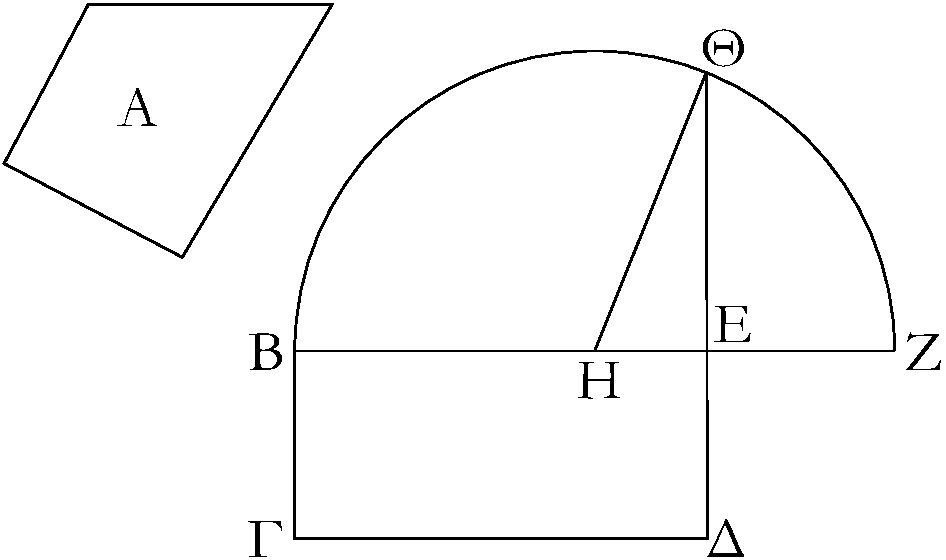
\includegraphics{Book02/fig14g.eps}}

\gr{Συνεστάτω γὰρ τῶ| Α ἐυθυγράμμῳ >ίσον παραλληλό\-γραμμον ὀρθογώνιον τὸ ΒΔ; εἰ μὲν ο>ῦν >ίση ἐστὶν ἡ ΒΕ τῆ| ΕΔ, γεγονὸξ
>ὰν ε>ίη τὸ ἐπιταθθέν. συνέσταται γὰρ τῶ| Α εὐθυγράμμῳ >ίσον
τετράγωνον τὸ ΒΔ; εἰ δὲ ο>ύ, μία τῶν ΒΕ, ΕΔ μείζων ἐστίν. >έστω
μείζων ἡ ΒΕ, καὶ ἐκβεβλήσθω ἐπὶ τὸ Ζ, καὶ κείσθω τῆ| ΕΔ >ίση
ἡ ΕΖ, καὶ τετμ\kern -.7pt  ήσθω ἡ ΒΖ δίθα κατὰ τὸ Η, καὶ κέντρῳ τῶ| Η,
διαστήματι δὲ ἑνὶ τῶν ΗΒ, ΗΖ ἡμικύκλιον γεγράφθω τὸ ΒJΖ, καὶ
ἐκβεβλήσθω ἡ ΔΕ ἐπὶ τὸ J, καὶ ἐπεζεύθθω ἡ ΗJ.}

\gr{Ἐπεὶ ο>ῦν εὐθεῖα ἡ ΒΖ τέτμ\kern -.7pt  ηται εἰξ μὲν >ίσα κατὰ τὸ Η, εἰξ
δὲ >άνισα κατὰ τὸ Ε, τὸ >άρα ὑπὸ τῶν ΒΕ, ΕΖ περιεχόμενον ὀρθογώνιον μετὰ τοῦ ἀπὸ τῆξ ΕΗ τετραγώνου >ίσον ἐστὶ
τῶ| ἀπὸ τῆξ ΗΖ τετραγώνῳ. >ίση δὲ ἡ ΗΖ τῆ| ΗJ; τὸ >άρα ὑπὸ τῶν ΒΕ, ΕΖ μετὰ τοῦ ἀπὸ τῆξ ΗΕ >ίσον ἐστὶ τῶ| ἀπὸ
τῆξ ΗJ. τῶ| δὲ ἀπὸ τῆξ ΗJ >ίσα ἐστὶ τὰ ἀπὸ τῶν JΕ, ΕΗ
τετράγωνα; τὸ >άρα ὑπὸ τῶν ΒΕ, ΕΖ μετὰ τοῦ ἀπὸ ΗΕ >ίσα ἐστὶ
τοῖξ ἀπὸ τῶν JΕ, ΕΗ. κοινὸν ἀφῃρήσθω τὸ ἀπὸ τῆξ ΗΕ
τετράγωνον; λοιπὸν
 >άρα τὸ ὑπὸ τῶν ΒΕ, ΕΖ περιεχόμενον >όρθογώνιον >ίσον ἐστὶ τῶ| ἀπὸ τῆξ ΕJ τετραγώνῳ.
ἀλλὰ τὸ ὑπὸ τῶν ΒΕ, ΕΖ τὸ ΒΔ ἐστιν; >ίση γὰρ ἡ ΕΖ τῆ| ΕΔ;
τὸ >άρα ΒΔ παραλληλόγραμμον >ίσον ἐστὶ τῶ| ἀπὸ τῆξ JΕ
τετραγώνῳ. >ίσον δὲ τὸ ΒΔ τῶ| Α εὐθυγράμμῳ. καὶ τὸ Α
>άρα εὐθύγραμμον >ίσον ἐστὶ τῶ| ἀπὸ τῆξ ΕJ
ἀναγραφησομένῳ τετραγώνῳ.}

\gr{Τῶ| >άρα δοθέντι εὐθυγράμμῳ  τῶ| Α >ίσον τετράγωνον συνέσταται τὸ ἀπὸ τῆξ ΕJ ἀναγραφησόμενον; <όπερ >έδει
ποιῆσαι.}}

\ParallelRText{
\begin{center}
{\large Proposition 14}
\end{center}

To construct a square equal to a given rectilinear figure.

Let $A$ be the given rectilinear figure. So it is required to construct a
square equal to the rectilinear figure $A$.

\epsfysize=2in
\centerline{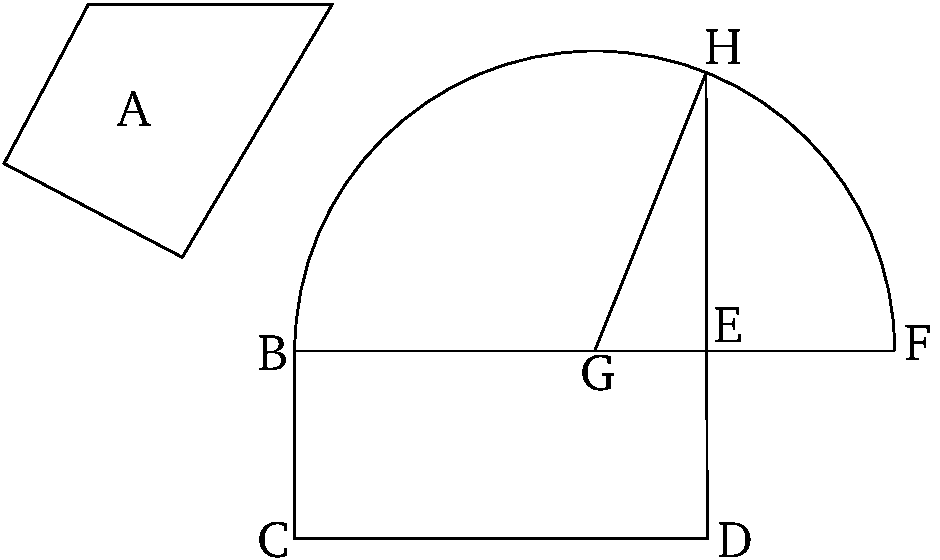
\includegraphics{Book02/fig14e.eps}}

For let the right-angled parallelogram $BD$,  equal to
the rectilinear figure $A$, be constructed  [Prop. 1.45]. Therefore, if $BE$ is equal to $ED$ then
that (which) was prescribed has taken place. For the square $BD$, equal to the rectilinear figure $A$,
has been constructed. And if not, (then)
one of the (straight-lines) $BE$ or $ED$ is greater (than the other). Let $BE$ be greater, and let it be
produced to $F$, and let $EF$ be made equal to $ED$ [Prop.~1.3].
And let $BF$ be cut in half at (point) $G$ [Prop.~1.10]. And, with center $G$, and
radius one of the (straight-lines) $GB$ or $GF$, let the semi-circle $BHF$ be drawn.
And let $DE$ be produced to $H$, and let $GH$ be joined.

Therefore, since the straight-line $BF$ has been cut---equally at $G$,
and unequally at $E$---the rectangle contained by $BE$ and $EF$, plus the
square on $EG$, is thus equal to the square on $GF$ [Prop.~2.5]. And $GF$ (is)
equal to $GH$. Thus, the (rectangle contained) by $BE$ and $EF$, plus the
(square) on $GE$, is equal to the (square) on $GH$. And the (sum of the) squares on $HE$ and $EG$  is equal to the (square)
on $GH$  [Prop.~1.47].
Thus, the (rectangle contained) by $BE$ and $EF$, plus the (square) on $GE$, is
equal to the (sum of the squares) on $HE$ and $EG$.
Let the square on $GE$ be taken from both. Thus, the remaining
rectangle contained by $BE$ and $EF$ is equal to the square
on $EH$. But, $BD$ is the (rectangle contained) by $BE$ and $EF$. For $EF$ (is)
equal to $ED$. Thus, the parallelogram $BD$ is equal to the square on $HE$.
And $BD$ (is) equal to the rectilinear figure $A$. Thus, the rectilinear figure
$A$ is also equal to the square (which) can be described on $EH$.

Thus, a 
square---(namely), that (which) can be described on $EH$---has been constructed, equal
to the given rectilinear figure $A$. (Which is) the very thing it was required to do.}
\end{Parallel}
